%\chapter{Spiral–Based Guidance Law and Multi-Agent Coordination}\label{ch:Spiral_Path}
\chapter[Spiral-Based Guidance Laws and Multi-Agent Spatial Coordination]{Spiral-Based Guidance Laws and Multi-Agent Spatial Coordination}\label{ch:Spiral_Path}
\section{Introduction and Motivation}\label{sec:ch_sp_intro}
In Chapter \ref{ch:Dubins_Path}, we formulated nonholonomic single-agent trajectory planning using Dubins-like geometric paths, demonstrating how adjusting a secondary turn radius $r_d$ satisfies simultaneous terminal approach angle and time-of-arrival constraints. While Dubins trajectories provide a minimal-length piecewise-constant acceleration framework, their discrete curvature jumps ($\kappa \in \{+1/r_m, 0, -1/r_d\}$) introduce jump discontinuities in the lateral acceleration profile. In high-speed atmospheric vehicles, agile robotic swarms, or guided precision interceptors, such step acceleration demands can excite unmodeled autopilot lag, induce mechanical chatter, or cause actuator saturation.

To achieve continuous curvature trajectories without discontinuities in lateral acceleration, \textbf{spiral-based path geometries} present a powerful alternative. Impact-angle-constrained guidance plays a pivotal role in modern cooperative engagements, where arriving at a target along specific spatial vectors maximizes warhead penetration, aligns directional sensors, or bypasses defensive countermeasure zones. Classical guidance laws—such as Pure Pursuit (PP) \cite{SHNEYDOR199847}, Deviated Pure Pursuit (DPP), and Proportional Navigation Guidance (PNG) \cite{SHNEYDOR1998101}— guarantee target interception but do not inherently enforce terminal impact angle constraints without demanding infinite terminal acceleration. Modified state-dependent Riccati equation (SDRE) laws \cite{ratnoo2009SDRE} and biased PNG schemes \cite{Kim2013} enforce impact angle constraints, but typically induce severe acceleration spikes near interception. Polynomial guidance approaches \cite{kim2013time} enforce boundary conditions but require rigid pre-computed trajectories that degrade under external wind perturbations or autopilot lags.

Generalized Archimedean spirals provide an attractive alternative: their polar geometry inherently embeds the desired terminal approach angle $\zeta$, while providing continuous, smooth curvature modulation throughout the engagement. However, existing spiral-based guidance schemes (e.g., \cite{tripathy2019archimedean}, \cite{mishra2024spiral}) operate under an unexamined assumption: they assume the initial geometric scaling parameter $\alpha_0$ yields a physically realizable path. If the initial launch geometry dictates a scaling factor below a critical reference threshold ($\alpha_0 < \alpha_{\text{ref}}$), the demanded lateral acceleration exceeds the physical actuator limits ($|a_p(t)| > a_{\max}$), causing catastrophic control saturation, leading to unacceptable miss-distances.

To overcome these challenges, this chapter presents a \emph{two-phase adaptive spiral guidance framework} that guarantees impact angle satisfaction while respecting strict physical actuator limits ($|a_p(t)| \le a_{\max}$). Furthermore, we extend this framework to multi-agent spatial coordination, using consensus in the spiral scaling parameter $\alpha$, over directed graphs to achieve distributed, sector-allocated coordinated interception. 

Although the framework presented in this chapter overcomes key physical and geometric limitations of classic Dubins-like strategies—extending them to multi-agent cooperative interception—we deliberately relax the requirement of strict simultaneous interception. Consequently, explicit terminal impact time constraints are not imposed, allowing the guidance strategy to prioritize angular sector alignment, actuator feasibility, and computational efficiency.

\subsection*{Summary of Chapter Contributions}
The primary analytical and algorithmic contributions of this chapter are:
\begin{enumerate}
    \item \textbf{Curvature Feasibility Analysis:} We derive exact closed-form expressions for the maximum curvature $\kappa_{\max} = f(\beta)/\alpha$ of generalized Archimedean spirals, establishing a sharp physical feasibility threshold $\alpha_{\text{ref}} \coloneqq v_p^2 f(\beta) / a_{\max}$.
    \item \textbf{Two-Phase Adaptive Scaling Control:} We formulate a two-phase guidance law that proactively adapts the scaling factor $\alpha(t) \to \alpha_{\text{ref}}$ during Phase 1 whenever $\alpha_0 < \alpha_{\text{ref}}$, eliminating lateral acceleration saturation before transitioning to Phase 2 terminal angle tracking.
    \item \textbf{Prescribed-Time Robust Error Suppression:} We integrate prescribed-time sliding mode control components into the adaptive spiral dynamics, proving finite-time error convergence $e(t) \to 0$ as $t \to T^*$ despite bounded process noise.
    \item \textbf{Directed Graph Multi-Agent Coordination:} We extend the single-agent framework to multi-agent swarms by executing directed chain consensus over the spiral parameter vector $\boldsymbol{\alpha}$, achieving synchronized, sector-allocated directional cooperative attacks across heterogeneous vehicle fleets.
\end{enumerate}
\section{Engagement Geometry and Kinematics}\label{sec:ch_sp_kinematics}
Consider the planar engagement geometry shown in Figure \ref{fig:ch_sp_eng_geometry}, where a pursuer (interceptor) engages a stationary target located at the origin $(x_t, y_t) = (0,0)$. The pursuer travels at constant speed $v_p > 0$ with heading angle $\gamma_p(t)$. Its control input is the lateral acceleration $a_p(t) \in \mathbb{R}$, subject to strict actuator saturation limits $|a_p(t)| \le a_{\max}$.

\begin{figure}[!ht]
	\centering
	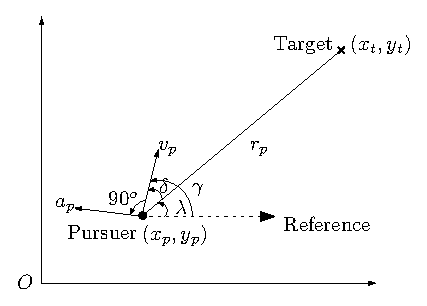
\includegraphics[width=0.75\textwidth, keepaspectratio]{6_Images/Eng_geom.eps}
	\caption{Planar engagement geometry between a pursuer and a stationary target in polar coordinates $(r_p, \lambda_p)$.}
	\label{fig:ch_sp_eng_geometry}
\end{figure}

The Cartesian kinematic equations of motion are:
\begin{equation}\label{eq:ch_sp_cartesian_kinematics}
	\dot{x}_p(t) = v_p \cos \gamma_p(t), \quad \dot{y}_p(t) = v_p \sin \gamma_p(t).
\end{equation}

To simplify geometric trajectory tracking, define the polar state variables:
\begin{itemize}
	\item $r_p(t) \coloneqq \sqrt{(x_t - x_p)^2 + (y_t - y_p)^2}$ : Range to target
	\item $\lambda_p(t) \coloneqq \operatorname{atan2}(y_t - y_p, x_t - x_p)$ : Line-of-sight (LOS) angle
	\item $\delta_p(t) \coloneqq \gamma_p(t) - \lambda_p(t)$ : Lead angle (look angle)
\end{itemize}

The nonholonomic engagement dynamics in polar coordinates are:
\begin{align}
	\dot{r}_p(t) &= -v_p \cos \delta_p(t) \label{eq:ch_sp_r_dot} \\
	r_p(t) \dot{\lambda}_p(t) &= -v_p \sin \delta_p(t) \label{eq:ch_sp_lambda_dot} \\
	\dot{\gamma}_p(t) &= \frac{a_p(t) + n(t)}{v_p}, \label{eq:ch_sp_gamma_dot}
\end{align}
where $n(t) \in \mathbb{R}$ represents bounded external process noise or wind disturbances ($|n(t)| \le N_0$).
In accordance with the physical constraints detailed in Section~\ref{sec:ch_DP_probform}, the commanded lateral acceleration is strictly bounded by $|a_M(t)| \le a^{\max}$ to avoid actuator saturation. Furthermore, the terminal boundary conditions are synthesized to meet the desired approach orientation $\theta_t$ as defined in Definition~\ref{def:ch_DP_impact_angle} and desired impact time as defined in ~\ref{def:ch_DP_impact_time}.
\begin{problem}\label{prob:ch_sp_main_problem}
Given an initial state configuration $\mathbf{x}(0) = [r_p(0), \lambda_p(0), \gamma_p(0)]^T$, constant flight speed $v_p$, maximum acceleration limit $a_{\max}$, and desired terminal approach angle $\zeta$, synthesize a continuous lateral acceleration guidance law $a_p(t)$ such that:
\begin{enumerate}
    \item \textbf{Target Interception:} The pursuer reaches the origin at terminal time $t_f$, satisfying $\lim_{t \to t_f} r_p(t) = 0$.
    \item \textbf{Impact Angle Satisfaction:} The velocity vector aligns precisely with the approach angle at interception: $\lim_{t \to t_f} \lambda_p(t) = \zeta$.
    \item \textbf{Actuator Feasibility:} The lateral acceleration strictly obeys the physical bound $|a_p(t)| \le a_{\max}$ for all $t \in [0, t_f]$.
\end{enumerate}
\end{problem}
\section{Archimedean Spiral Trajectory Framework}\label{sec:ch_sp_spiral_framework}
\leavevmode\par\noindent
To satisfy Problem \ref{prob:ch_sp_main_problem} without involving high-order polynomial calculations, or discontinuous step acceleration commands, we formulate trajectory generation using a generalized Archimedean spiral geometry.
\subsection{Geometric Parameterization and Chief Merits of Proposed Strategy}\label{subsec:ch_sp_spiral_def}

We parameterize the path of the pursuer in polar space $(r, \lambda)$ around the generalized Archimedean spiral:
\begin{equation}\label{eq:ch_sp_spiral_def}
	r(\lambda) = \alpha (\lambda - \zeta)^\beta, \quad \text{for } \lambda \ge \zeta,
\end{equation}
where $\zeta$ is the designated terminal impact angle, $\beta \in (0, 1]$ is a fixed geometric shape exponent, and $\alpha > 0$ is the spatial scaling parameter.

This parameterization introduces two fundamental geometric properties for guidance of nonholonomic vehicles which are very appealing:

\begin{enumerate}
    \item \textbf{Implicit Terminal Angle Alignment:} As relative range vanishes ($r \to 0$), the polar angle asymptotically approaches the target angle ($\lambda \to \zeta$). Because the tangent to spiral \eqref{eq:ch_sp_spiral_def} aligns with $\zeta$ at the origin, terminal impact angle satisfaction ($\lambda_p(t_f) = \zeta$) is intrinsically embedded into the spatial geometry, eliminating the need for high-gain terminal corrective steering.
    
    \item \textbf{Zero Terminal Acceleration Demand:} The geometry of the spiral \eqref{eq:ch_sp_spiral_def} dictates that path curvature $\kappa(\lambda)$ approaches zero as $\lambda \to \zeta$. Consequently, the commanded lateral acceleration $a_p = v_p^2 \kappa$ vanishes naturally at interception ($a_p(t_f) = 0$), thus avoiding terminal control saturation and autopilot chattering.
\end{enumerate}
\subsection{Path Curvature Analysis and Critical Feasibility Threshold}\label{subsec:ch_sp_curvature_analysis}

While the spiral geometry inherently satisfies terminal angle constraints, its physical realizability depends on whether the required path curvature exceeds the vehicle's turn capability ($a_{\max} / v_p^2$) or not. 

The path curvature $\kappa(\lambda)$ of a polar curve $r(\lambda)$ is governed by the classical relation:
\begin{equation}\label{eq:ch_sp_kappa_general_formula}
	\kappa(\lambda) = \frac{\big|r^2 + 2(r')^2 - r r''\big|}{\left( r^2 + (r')^2 \right)^{3/2}},
\end{equation}
where $r' \coloneqq \frac{\mathrm{d}r}{\mathrm{d}\lambda}$ and $r'' \coloneqq \frac{\mathrm{d}^2 r}{\mathrm{d}\lambda^2}$.

Differentiating parameterization \eqref{eq:ch_sp_spiral_def} with respect to $\lambda$ yields:
\begin{equation}\label{eq:ch_sp_spiral_derivatives}
    r' = \alpha \beta (\lambda - \zeta)^{\beta-1}, \quad r'' = \alpha \beta (\beta-1) (\lambda - \zeta)^{\beta-2}.
\end{equation}

Defining the angular offset $\theta \coloneqq \lambda - \zeta > 0$, substituting $r(\theta) = \alpha \theta^\beta$ and its derivatives \eqref{eq:ch_sp_spiral_derivatives} into \eqref{eq:ch_sp_kappa_general_formula} gives:
\begin{align}\label{eq:ch_sp_kappa_explicit_derivation}
	\kappa(\theta) &= \frac{\left| \alpha^2 \theta^{2\beta} + 2 \alpha^2 \beta^2 \theta^{2\beta-2} - \alpha^2 \beta(\beta-1) \theta^{2\beta-2} \right|}{\left( \alpha^2 \theta^{2\beta} + \alpha^2 \beta^2 \theta^{2\beta-2} \right)^{3/2}} \nonumber \\
	&= \frac{\alpha^2 \theta^{2\beta-2} \left| \theta^2 + \beta^2 + \beta \right|}{\alpha^3 \theta^{3\beta-3} \left( \theta^2 + \beta^2 \right)^{3/2}} \nonumber \\
	&= \frac{1}{\alpha} \cdot \frac{\theta^{1-\beta} (\beta^2 + \beta + \theta^2)}{(\beta^2 + \theta^2)^{3/2}}.
\end{align}

We isolate the dimensionless, scale-independent shape curvature function $f(\beta, \theta)$:
\begin{equation}\label{eq:ch_sp_f_beta_theta_def}
    f(\beta, \theta) \coloneqq \frac{\theta^{1-\beta} (\beta^2 + \beta + \theta^2)}{(\beta^2 + \theta^2)^{3/2}}, \implies \kappa(\theta) = \frac{f(\beta, \theta)}{\alpha}.
\end{equation}

To find the peak curvature along the trajectory, we differentiate $f(\beta, \theta)$ with respect to $\theta$ and solve $\frac{\partial f}{\partial \theta} = 0$, which yields the critical angular offset $\theta^*$:
\begin{equation}\label{eq:ch_sp_critical_theta}
    \theta^* = \sqrt{\sqrt{3\beta^2+1} - 1 - \beta^2}.
\end{equation}

Evaluating $f(\beta) \coloneqq \max_\theta f(\beta, \theta) = f(\beta, \theta^*)$ yields the maximum shape curvature constant:
\begin{equation}\label{eq:ch_sp_f_beta_max}
	f(\beta) = \frac{\sqrt{3\beta^2+1} + \beta - 1}{\left( \sqrt{3\beta^2+1} - 1 - \beta^2 \right)^{\frac{\beta-1}{2}} \left( \sqrt{3\beta^2+1} - 1 \right)^{3/2}}.
\end{equation}

Consequently, the peak curvature $\kappa_{\max}$ experienced along an Archimedean spiral trajectory is inversely proportional to the spatial scaling parameter $\alpha$:
\begin{equation}\label{eq:ch_sp_kappa_max}
	\kappa_{\max} = \frac{f(\beta)}{\alpha}.
\end{equation}

Since commanded lateral acceleration is related to curvature via $a_{\text{cmd}} = v_p^2 \kappa$, the maximum acceleration required to track the spiral is:
\begin{equation}\label{eq:ch_sp_acmd_max}
    a_{\max, \text{cmd}} = \frac{v_p^2 f(\beta)}{\alpha}.
\end{equation}

The variation of path curvature $\kappa(\theta)$ across different scaling values $\alpha$ for a fixed shape exponent $\beta = 0.5$ is illustrated in Figure \ref{fig:ch_sp_curv_vs_angle}.

\begin{figure}[!ht]
	\centering
	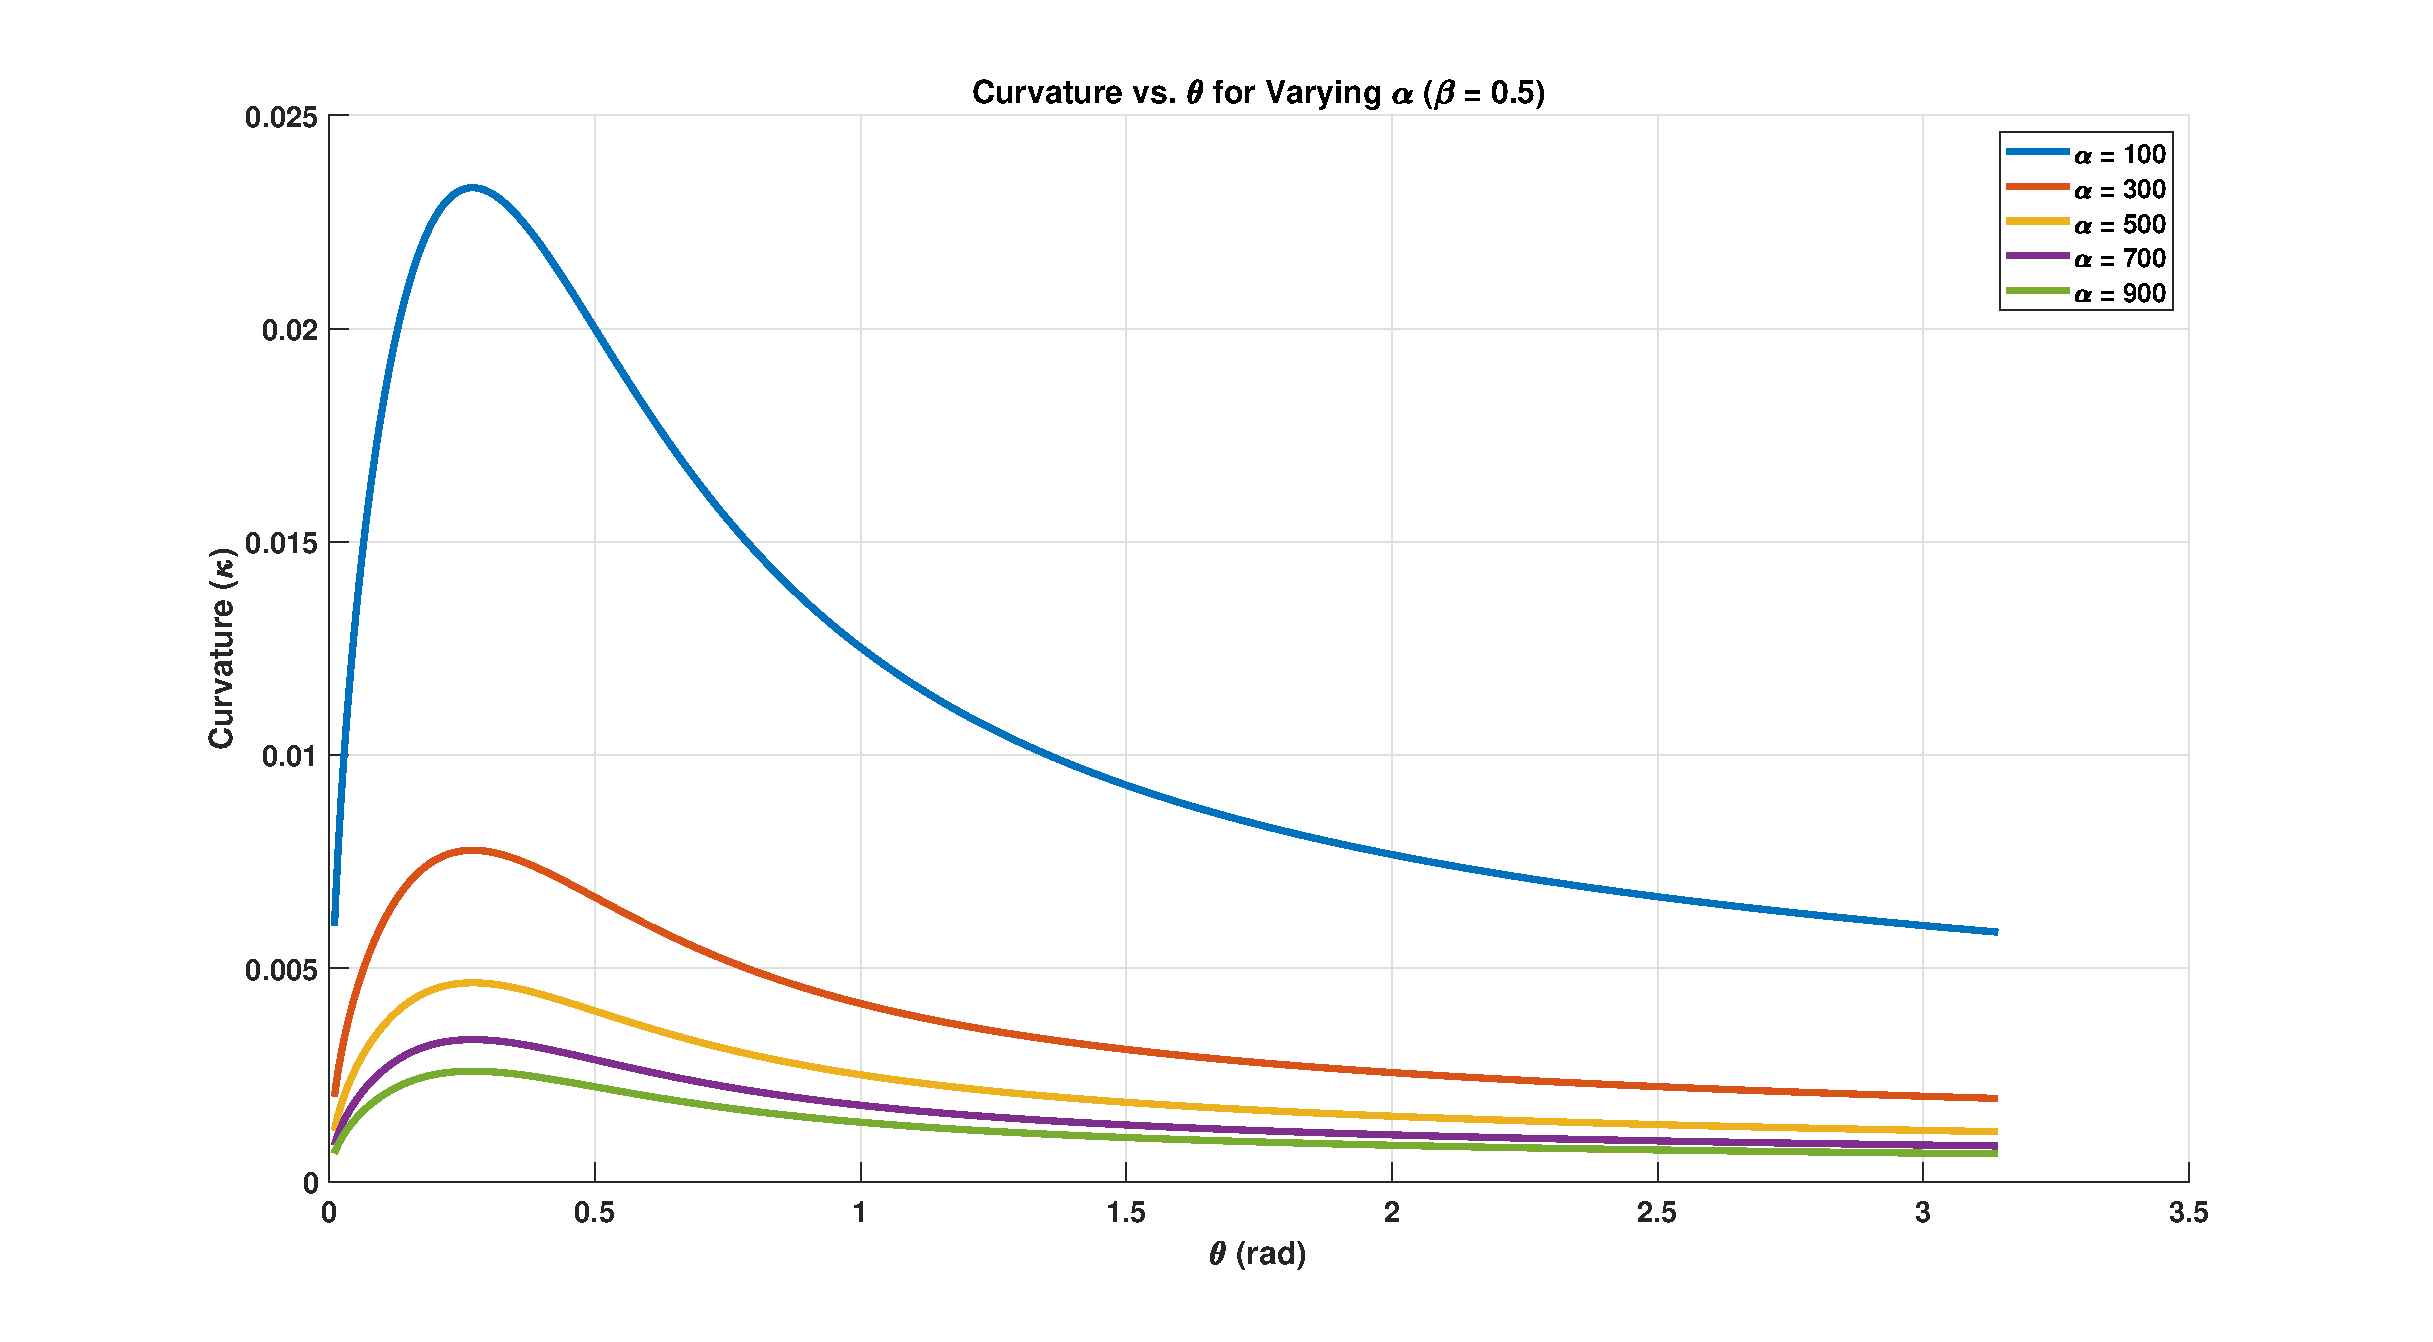
\includegraphics[width=0.75\textwidth]{6_Images/CurvVsAngle_FixedBeta_VaryingAlpha.eps}
	\caption{Path curvature $\kappa(\theta)$ versus angular offset $\theta = \lambda - \zeta$ for fixed exponent $\beta = 0.5$ across varying scaling factors $\alpha$. Smaller values of $\alpha$ significantly amplify peak trajectory curvature.}
	\label{fig:ch_sp_curv_vs_angle}
\end{figure}

\subsection{Physical Infeasibility of Unadapted Spiral Guidance}\label{subsec:ch_sp_infeasibility_proof}
To guarantee that the commanded lateral acceleration strictly respects actuator limits ($a_{\max, \text{cmd}} \le a_{\max}$), the scaling parameter $\alpha$ must satisfy $\alpha \ge \alpha_{\text{ref}}$, where the critical physical reference threshold $\alpha_{\text{ref}}$ is defined as:
\begin{equation}\label{eq:ch_sp_alpha_ref}
	\alpha_{\text{ref}} \coloneqq \frac{v_p^2 f(\beta)}{a_{\max}}.
\end{equation}

In standard unadapted spiral guidance laws (e.g., \cite{mishra2024spiral}), the scaling parameter $\alpha_0$ is statically computed from initial launch conditions:
\begin{equation}\label{eq:ch_sp_initial_alpha}
    \alpha_0 = \frac{r_p(0)}{\big(\lambda_p(0) - \zeta\big)^\beta}.
\end{equation}

Because initial range $r_p(0)$ and launch angles are dictated by arbitrary engagement geometry rather than actuator constraints, $\alpha_0$ frequently falls below the critical threshold ($\alpha_0 < \alpha_{\text{ref}}$). When $\alpha_0 < \alpha_{\text{ref}}$, the peak curvature demand exceeds $a_{\max} / v_p^2$, driving the actuators into saturation.

Figure \ref{fig:ch_sp_kushagra_breakdown} illustrates the catastrophic control breakdown that occurs under unadapted spiral guidance when $\alpha_0 < \alpha_{\text{ref}}$. Actuator saturation ($|a_p| = 30g$) prevents the pursuer from following the nominal spiral, causing large miss distances and trajectory degradation.

\begin{figure}[!ht]
	\centering
	\begin{subfigure}[b]{0.7\textwidth}
		\centering
		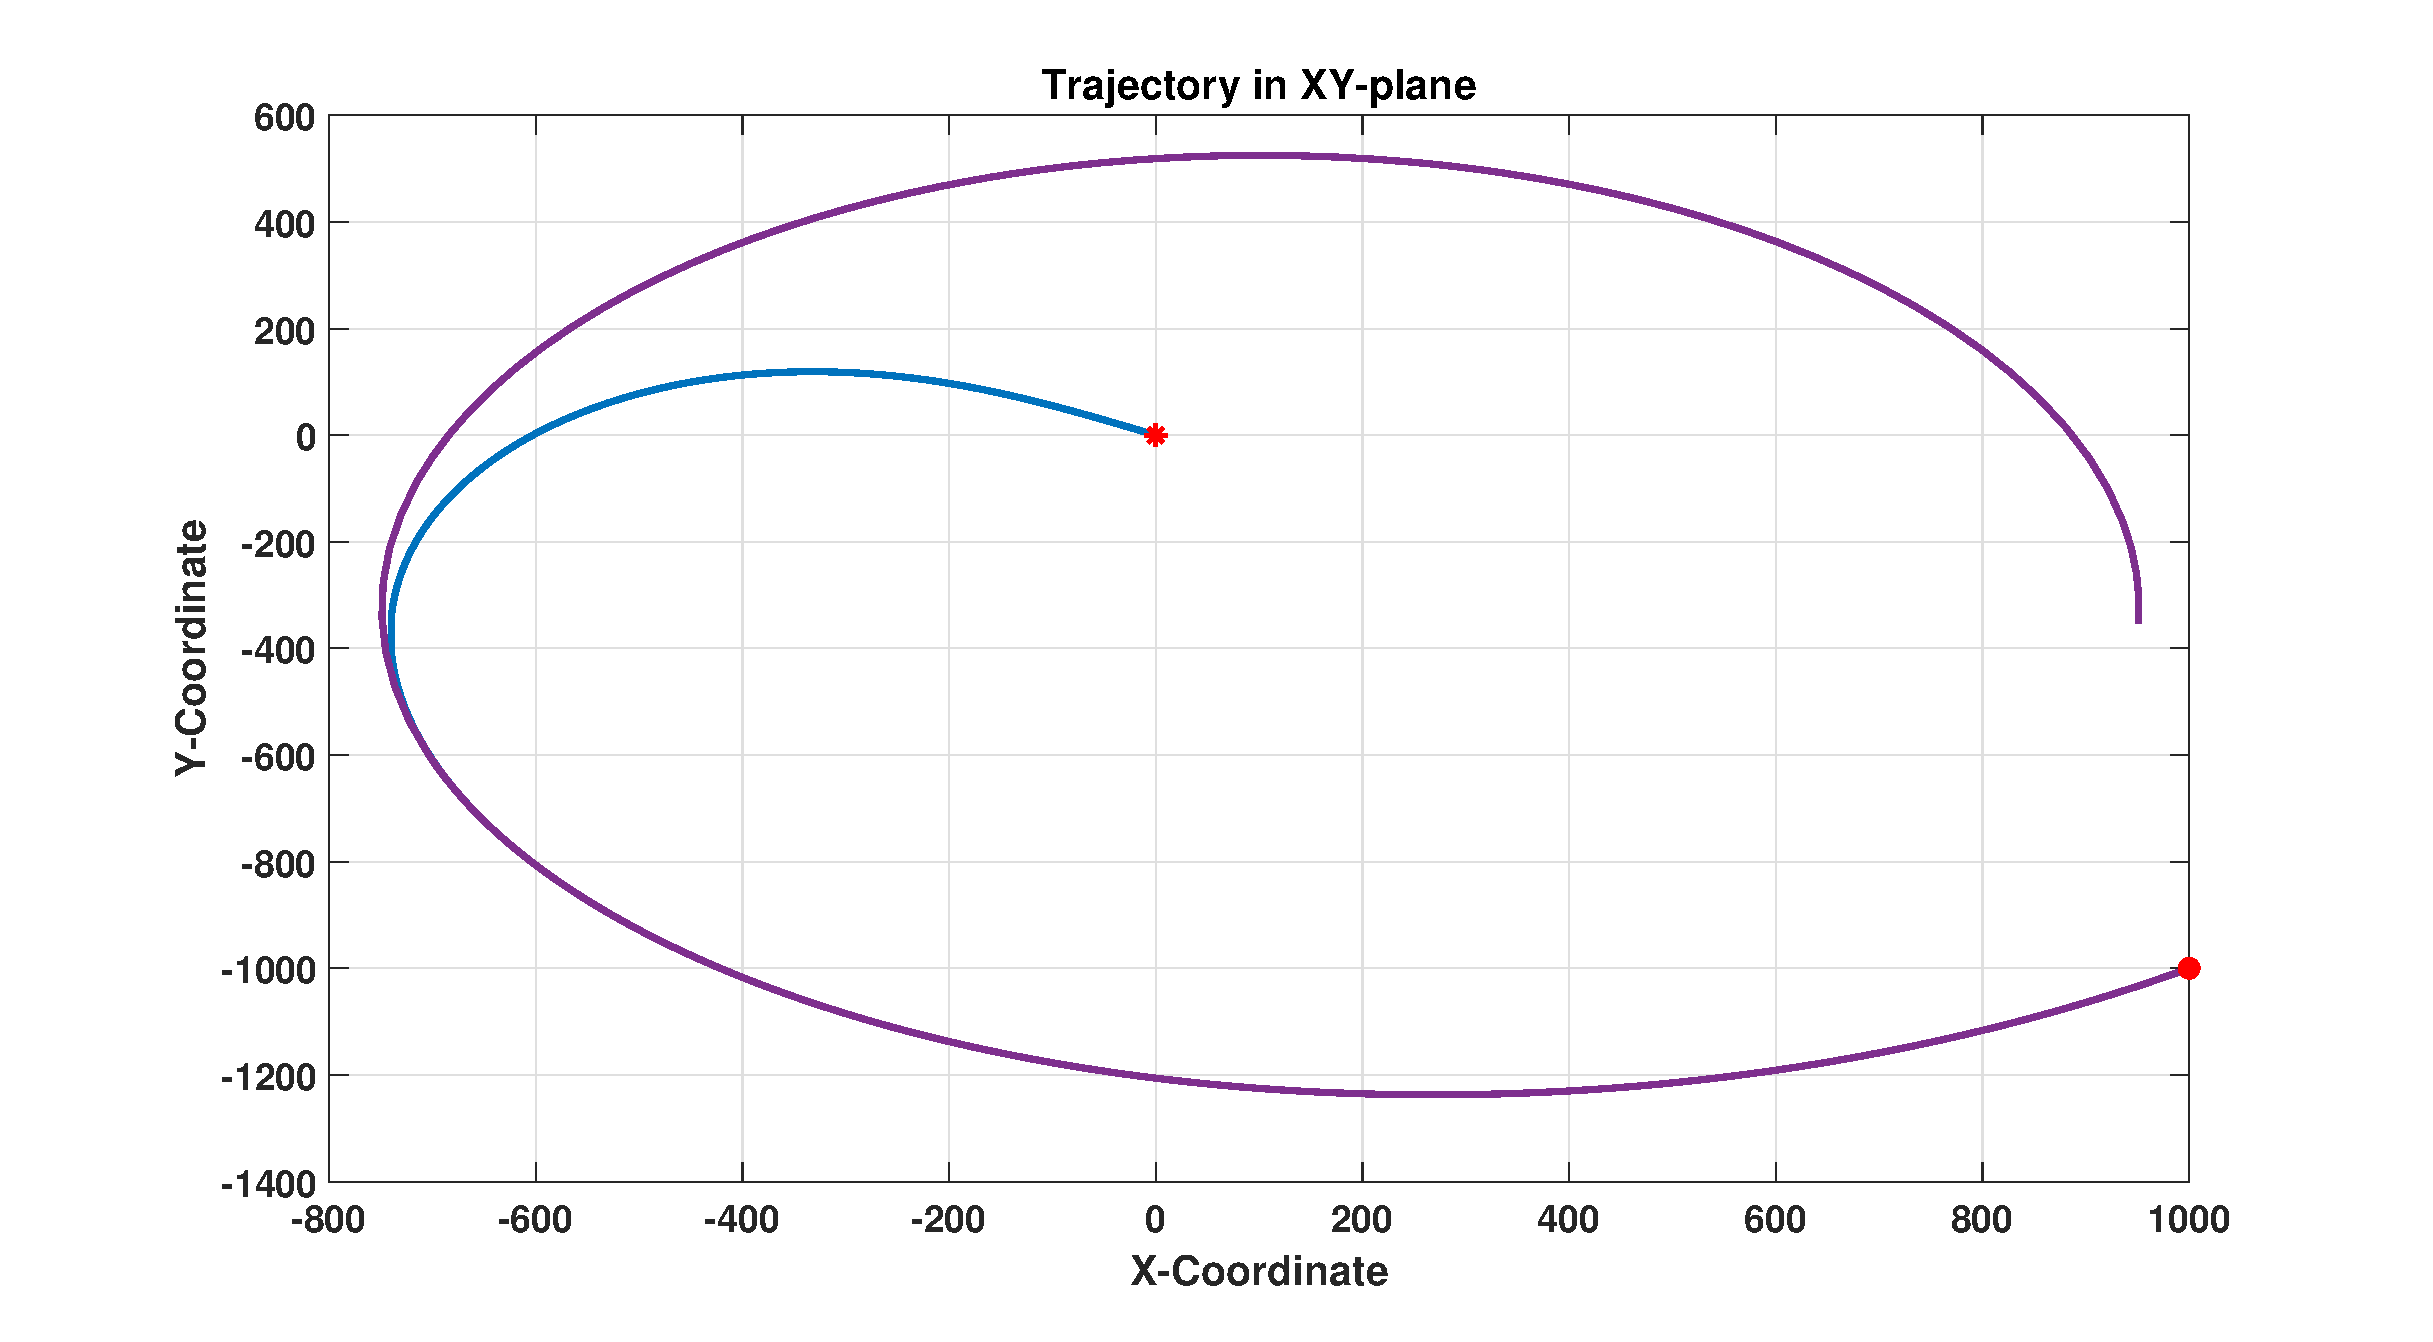
\includegraphics[width=\textwidth]{6_Images/Trajectory_Kushagra.eps}
		\caption{Interception trajectories with and without acceleration bounds.}
		\label{fig:ch_sp_kushagra_traj}
	\end{subfigure}
	\hfill
	\begin{subfigure}[b]{0.7\textwidth}
		\centering
		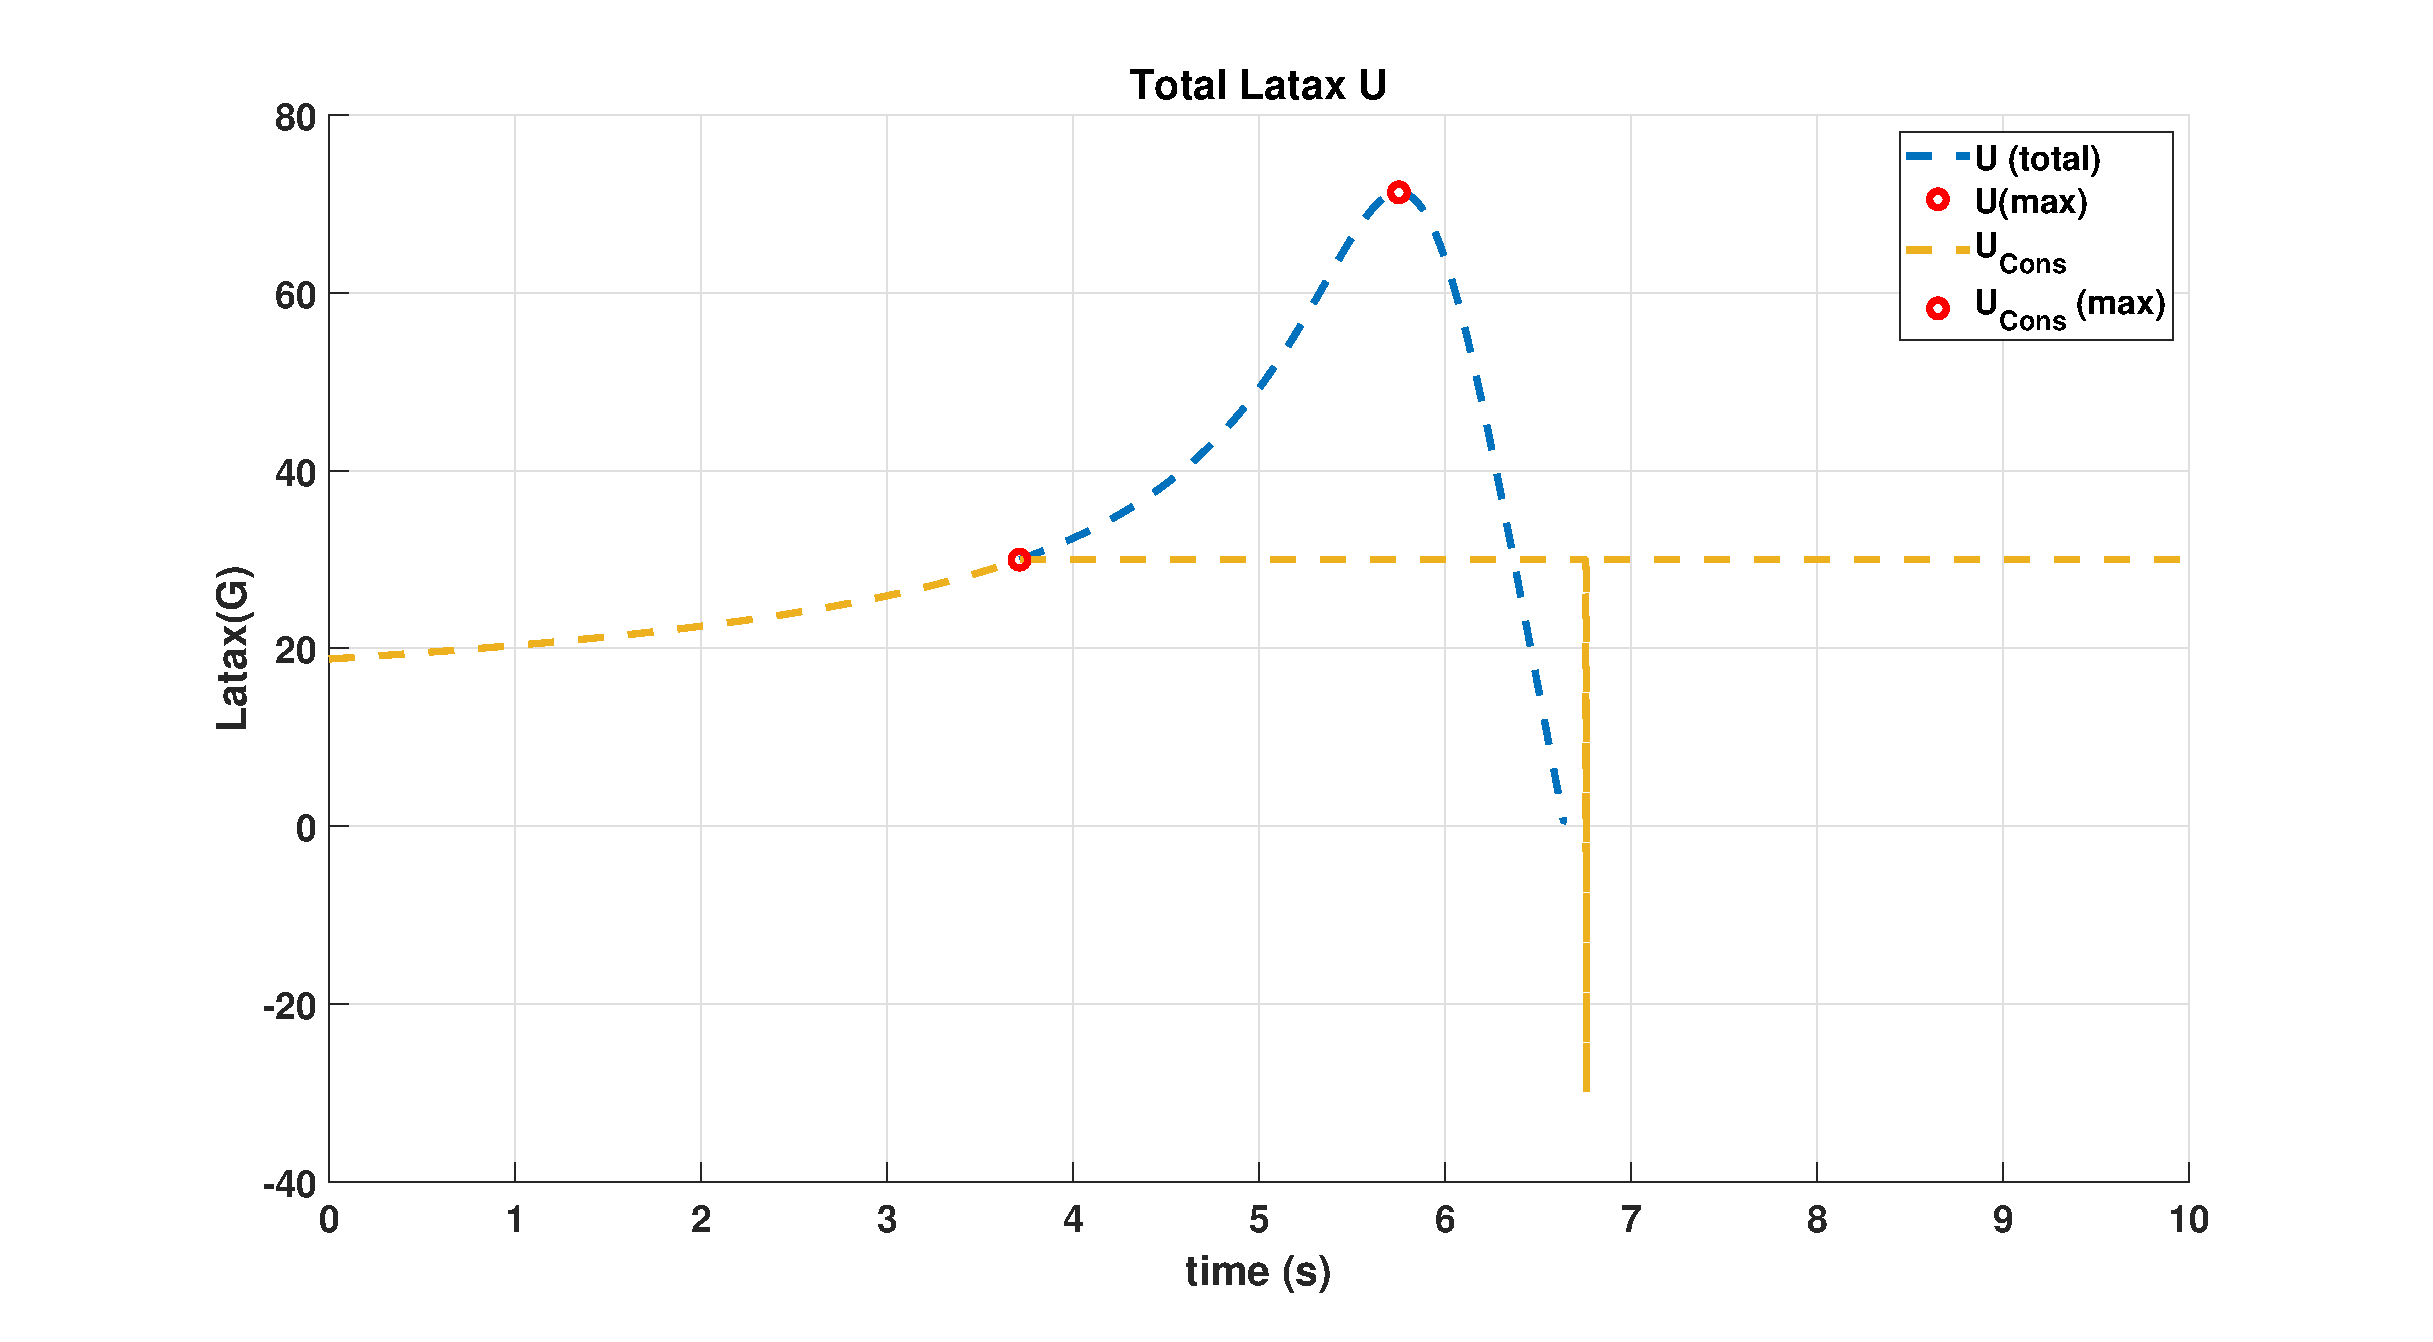
\includegraphics[width=\textwidth]{6_Images/Latax_Kushagra.eps}
		\caption{Commanded versus saturated lateral acceleration.}
		\label{fig:ch_sp_kushagra_latax}
	\end{subfigure}
	\caption{Demonstration of control breakdown in unadapted spiral guidance \cite{mishra2024spiral} when initial geometry dictates $\alpha_0 < \alpha_{\text{ref}}$. Actuator saturation ($30g$) leads to severe trajectory distortion.}
	\label{fig:ch_sp_kushagra_breakdown}
\end{figure}

This vulnerability necessitates the \emph{Two-Phase Adaptive Guidance Framework} formulated in Section \ref{sec:ch_sp_adaptive_guidance} next, which dynamically adapts $\alpha(t) \to \alpha_{\text{ref}}$ to guarantee physical feasibility before enforcing terminal angle tracking.
The control objective is to design the lateral acceleration command $a_p(t)$ such that the pursuer intercepts the target ($r_p(t_f) = 0$) at a specified terminal approach angle $\zeta$:
\begin{equation}\label{eq:ch_sp_terminal_objective}
	\lim_{t \to t_f} \lambda_p(t) = \zeta, \quad \text{subject to } |a_p(t)| \le a_{\max}, \quad \forall t \in [0, t_f].
\end{equation}
\section{Two-Phase Adaptive Guidance Law Synthesis}\label{sec:ch_sp_adaptive_guidance}

As established in Section~\ref{subsec:ch_sp_curvature_analysis}, standard spiral guidance schemes suffer from control saturation, whenever the initial geometric configuration enforces a scaling parameter smaller than the critical feasibility threshold ($\alpha_0 < \alpha_{\text{ref}}$). To guarantee precise terminal impact angle alignment—as defined in Definition~\ref{def:ch_DP_impact_angle}—without exceeding the physical actuator saturation limits detailed in Section~\ref{sec:ch_DP_probform} ($|a_p(t)| \le a_{\max}$), we synthesize a novel two-phase adaptive guidance law.

The overarching design philosophy separates the engagement into two distinct functional regimes:
\begin{enumerate}
    \item \textbf{Phase 1 (Feasibility-Seeking Mode):} When $\alpha(t) < \alpha_{\text{ref}}$, the guidance law dynamically updates the scaling parameter $\alpha(t) \to \alpha_{\text{ref}}$ online via dynamic feedback while steering the vehicle toward the feasible spiral manifold.
    \item \textbf{Phase 2 (Terminal Guidance Mode):} Once $\alpha(t)$ reaches the feasibility threshold $\alpha_{\text{ref}}$, adaptation is frozen ($\dot{\alpha} = 0$), and the guidance protocol smoothly transitions to pure geometric spiral tracking, ensuring $a_p(t_f) = 0$ and $\lambda_p(t_f) = \zeta$.
\end{enumerate}
\subsection{Composite Error Vector Formulation}\label{subsec:ch_sp_error_formulation}

To simultaneously regulate trajectory shape and geometric scaling, we formulate a composite error tracking metric $e(t) \in \mathbb{R}$:
\begin{equation}\label{eq:ch_sp_composite_error}
	e(t) \coloneqq e_{\text{shape}}(t) + k_r e_{\text{scale}}(t),
\end{equation}
where $k_r > 0$ is a scalar gain balancing angular shape alignment against range-scale tracking.

The individual error components are defined as:
\begin{align}
	e_{\text{shape}}(t) &\coloneqq \delta_p(t) - \tan^{-1}\left( \frac{\lambda_p(t) - \zeta}{\beta} \right), \label{eq:ch_sp_e_shape} \\
	e_{\text{scale}}(t) &\coloneqq r_p(t) - \alpha(t) (\lambda_p(t) - \zeta)^\beta. \label{eq:ch_sp_e_scale}
\end{align}

Notice that driving $e_{\text{shape}}(t) \to 0$ forces the lead angle $\delta_p(t)$ to align with the tangent manifold of the Archimedean spiral, whereas driving $e_{\text{scale}}(t) \to 0$ enforces exact adherence to the desired spatial range profile $r(\lambda)$.
\subsection{Phase 1: Feasibility-Seeking Guidance Mode ($\alpha(t) < \alpha_{\text{ref}}$)}\label{subsec:ch_sp_phase1}

During the initial phase of engagement, if the initial launch geometry yields an infeasible scaling factor ($\alpha_0 < \alpha_{\text{ref}}$), the parameter $\alpha(t)$ is driven dynamically toward $\alpha_{\text{ref}}$ using proportional feedback:
\begin{equation}\label{eq:ch_sp_alpha_dot_phase1}
	\dot{\alpha}(t) = K_p \big(\alpha_{\text{ref}} - \alpha(t)\big), \quad \alpha(0) = \alpha_0, \quad K_p > 0.
\end{equation}

To synthesize the lateral acceleration control command $a_p(t)$, we evaluate the time derivative of the composite error vector \eqref{eq:ch_sp_composite_error} along the relative polar kinematic equations \eqref{eq:ch_sp_r_dot}--\eqref{eq:ch_sp_lambda_dot}:
\begin{align}\label{eq:ch_sp_e_dot_derivation}
	\dot{e}(t) &= \dot{e}_{\text{shape}}(t) + k_r \dot{e}_{\text{scale}}(t) \nonumber \\
	&= \left( \dot{\gamma}_p - \dot{\lambda}_p - \frac{\frac{\dot{\lambda}_p}{\beta}}{1 + \left(\frac{\lambda_p - \zeta}{\beta}\right)^2} \right) + k_r \left( \dot{r}_p - \dot{\alpha}(\lambda_p - \zeta)^\beta - \alpha \beta (\lambda_p - \zeta)^{\beta-1} \dot{\lambda}_p \right).
\end{align}

Substituting the flight path angle dynamics $\dot{\gamma}_p = \frac{a_p + n}{v_p}$ and the LOS rate expression $\dot{\lambda}_p = -\frac{v_p \sin \delta_p}{r_p}$ into \eqref{eq:ch_sp_e_dot_derivation} yields:
\begin{align}\label{eq:ch_sp_e_dot_expanded}
	\dot{e}(t) &= \frac{a_p + n}{v_p} + \frac{v_p \sin \delta_p}{r_p} \left( 1 + \frac{1}{\beta \left( 1 + \frac{(\lambda_p - \zeta)^2}{\beta^2} \right)} \right) \nonumber \\
	&\quad + k_r \left( -v_p \cos \delta_p - \dot{\alpha}(\lambda_p - \zeta)^\beta + \frac{\alpha \beta v_p \sin \delta_p (\lambda_p - \zeta)^{\beta-1}}{r_p} \right).
\end{align}

To invert the non-autonomous kinematic drift terms and guarantee finite-time error convergence in the presence of bounded process noise $|n(t)| \le N_0$, the lateral acceleration $a_p(t)$ is decomposed into three distinct feedback terms:
\begin{equation}\label{eq:ch_sp_ap_phase1}
	a_p(t) = a_{\text{shape}}(t) + a_{\text{scale}}(t) + a_{\text{PT}}(t),
\end{equation}
where:
\begin{align}
	a_{\text{shape}}(t) &= -\frac{v_p^2 \sin \delta_p}{r_p} \left( 1 + \frac{1}{\beta \left( 1 + \frac{(\lambda_p - \zeta)^2}{\beta^2} \right)} \right), \label{eq:ch_sp_ashape} \\
	a_{\text{scale}}(t) &= k_r v_p \left( v_p \cos \delta_p + \dot{\alpha} (\lambda_p - \zeta)^\beta - \frac{\alpha \beta v_p \sin \delta_p (\lambda_p - \zeta)^{\beta-1}}{r_p} \right). \label{eq:ch_sp_ascale}
\end{align}

The third term, $a_{\text{PT}}(t)$, is a prescribed-time robust control command designed to drive $e(t) \to 0$ within a pre-specified time frame $T^* > 0$, regardless of initial conditions or disturbance magnitude:
\begin{equation}\label{eq:ch_sp_aPT}
	a_{\text{PT}}(t) = -v_p \left( \frac{c_1 |e|^{\alpha_1}}{\tau^{\mu_1}(t)} + \frac{c_2 |e|^{\alpha_2}}{\tau^{\mu_2}(t)} \right) \operatorname{sgn}(e), \quad \tau(t) \coloneqq T^* - t,
\end{equation}
where $c_1, c_2 > 0$ are design gains, $\mu_1, \mu_2 \ge 1$ dictate convergence power, and $0 < \alpha_1 < 1 < \alpha_2$ ensures bi-limit uniform finite-time stability.
\subsection{Phase 2: Terminal Guidance Mode ($\alpha(t) \ge \alpha_{\text{ref}}$) and Phase Transition Logic}\label{subsec:ch_sp_phase2}
The transition between operational modes is governed by a continuous condition check on the scaling parameter $\alpha(t)$.

\begin{figure}[!ht]
	\centering
	\begin{tikzpicture}[node distance=2.2cm, auto, >=stealth, thick]
		% Styles
		\tikzstyle{block} = [draw, fill=blue!10, rectangle, minimum height=3em, minimum width=10em, rounded corners, align=center]
		\tikzstyle{decision} = [draw, fill=orange!15, diamond, aspect=2, align=center]
		\tikzstyle{line} = [draw, ->, thick]
		
		% Nodes
		\node [block] (init) {\textbf{Initialize Engagement}\\ Compute $\alpha_0 = \frac{r_p(0)}{(\lambda_p(0)-\zeta)^\beta}$};
		\node [decision, below of=init, node distance=2.2cm] (check) {$\alpha(t) \ge \alpha_{\text{ref}}$ ?};
		\node [block, left of=check, node distance=6.8cm] (phase1) {\textbf{Phase 1: Feasibility Mode}\\ Dynamic Adaptation: $\dot{\alpha} = K_p(\alpha_{\text{ref}}-\alpha)$\\ Apply $a_p = a_{\text{shape}} + a_{\text{scale}} + a_{\text{PT}}$};
		\node [block, below of=check, node distance=2.5cm] (phase2) {\textbf{Phase 2: Terminal Mode}\\ Freeze Adaptation: $\dot{\alpha} = 0 \implies \alpha = \alpha_{\text{ref}}$\\ Geometric Tracking: $\tan \delta_p = \frac{\lambda_p - \zeta}{\beta}$};
		
		% Paths
		\path [line] (init) -- (check);
		\path [line] (check) -- node [above] {No} (phase1);
		\path [line] (phase1) |- (init);
		\path [line] (check) -- node [right] {Yes} (phase2);
	\end{tikzpicture}
	\caption{Flowchart illustrating the operational switching logic of the Two-Phase Adaptive Guidance Law.}
	\label{fig:ch_sp_switching_logic}
\end{figure}

As depicted in Figure~\ref{fig:ch_sp_switching_logic}, once the online dynamic update \eqref{eq:ch_sp_alpha_dot_phase1} drives the scaling factor to the physical reference threshold $\alpha_{\text{ref}}$, the parameter adaptation is frozen:
\begin{equation}\label{eq:ch_sp_alpha_dot_phase2}
	\dot{\alpha}(t) = 0 \implies \alpha(t) = \alpha_{\text{ref}}, \quad \forall t \ge t_{\text{switch}}.
\end{equation}

Upon entering Phase 2, composite tracking error $e(t)$ has converged to zero ($e_{\text{shape}} = 0, e_{\text{scale}} = 0$). Consequently, system control simplifies directly to standard geometric spiral tracking:
\begin{equation}\label{eq:ch_sp_phase2_geometric_law}
	\tan \delta_p(t) = \frac{\lambda_p(t) - \zeta}{\beta}.
\end{equation}

By freezing $\alpha(t)$ at $\alpha_{\text{ref}}$, the vehicle is guaranteed to navigate along a trajectory whose peak curvature demand strictly satisfies $\kappa_{\max} \le a_{\max} / v_p^2$. Thus, Phase 2 ensures exact, unsaturated convergence to the desired terminal impact angle $\lim_{t \to t_f} \lambda_p(t) = \zeta$ while maintaining zero terminal acceleration demand ($a_p(t_f) = 0$).

\section{Single-Agent Simulation Results and Physical Analysis}\label{sec:ch_sp_single_sims}

To rigorously evaluate the performance of the proposed two-phase adaptive guidance law, numerical simulations were conducted for a single pursuer engaging a stationary target located at the origin $\mathcal{O}(0,0)$.

\subsection{Simulation Setup and Initial Infeasibility Analysis}\label{subsec:ch_sp_sim_setup}

The engagement parameters and vehicle physical limits are configured as follows:
\begin{itemize}
    \item \textbf{Kinematic States:} Initial Cartesian position $(x_p(0), y_p(0)) = (1000\text{ m}, -1000\text{ m})$, constant flight speed $v_p = 500\text{ m/s}$, and initial lead angle $\delta_p(0) = \pi/6$ ($30^\circ$).
    \item \textbf{Terminal Objective:} Desired impact angle $\zeta = -\pi/4$ ($-45^\circ$).
    \item \textbf{Actuator and Geometry Parameters:} Maximum lateral acceleration $a_{\max} = 30g = 294.3\text{ m/s}^2$ and spiral shape exponent $\beta = 0.5$.
\end{itemize}

Evaluating the initial polar coordinates yields $r_p(0) = 1414.2\text{ m}$ and $\lambda_p(0) = 135^\circ$ ($2.3562\text{ rad}$). Using \eqref{eq:ch_sp_initial_alpha}, the initial unadapted geometric scaling parameter is:
\begin{equation}\label{eq:ch_sp_sim_alpha0}
    \alpha_0 = \frac{r_p(0)}{\big(\lambda_p(0) - \zeta\big)^\beta} = \frac{1414.2}{(2.3562 - (-0.7854))^{0.5}} = 797.88.
\end{equation}

Evaluating the critical physical reference threshold via \eqref{eq:ch_sp_alpha_ref} yields $\alpha_{\text{ref}} = \frac{v_p^2 f(0.5)}{a_{\max}} = 1241.5$. Because $\alpha_0 = 797.88 < \alpha_{\text{ref}}$, any conventional unadapted guidance law would demand peak lateral acceleration far exceeding $30g$, leading to immediate control saturation and interception failure.
\subsection{Spatial Kinematics and State Convergence}\label{subsec:ch_sp_spatial_results}

Figure~\ref{fig:ch_sp_trajectory_and_states} illustrates the spatial pursuit trajectory alongside the time evolution of the relative polar states under the proposed adaptive guidance scheme.

\begin{figure}[!ht]
	\centering
	\begin{subfigure}[b]{\textwidth}
		\centering
		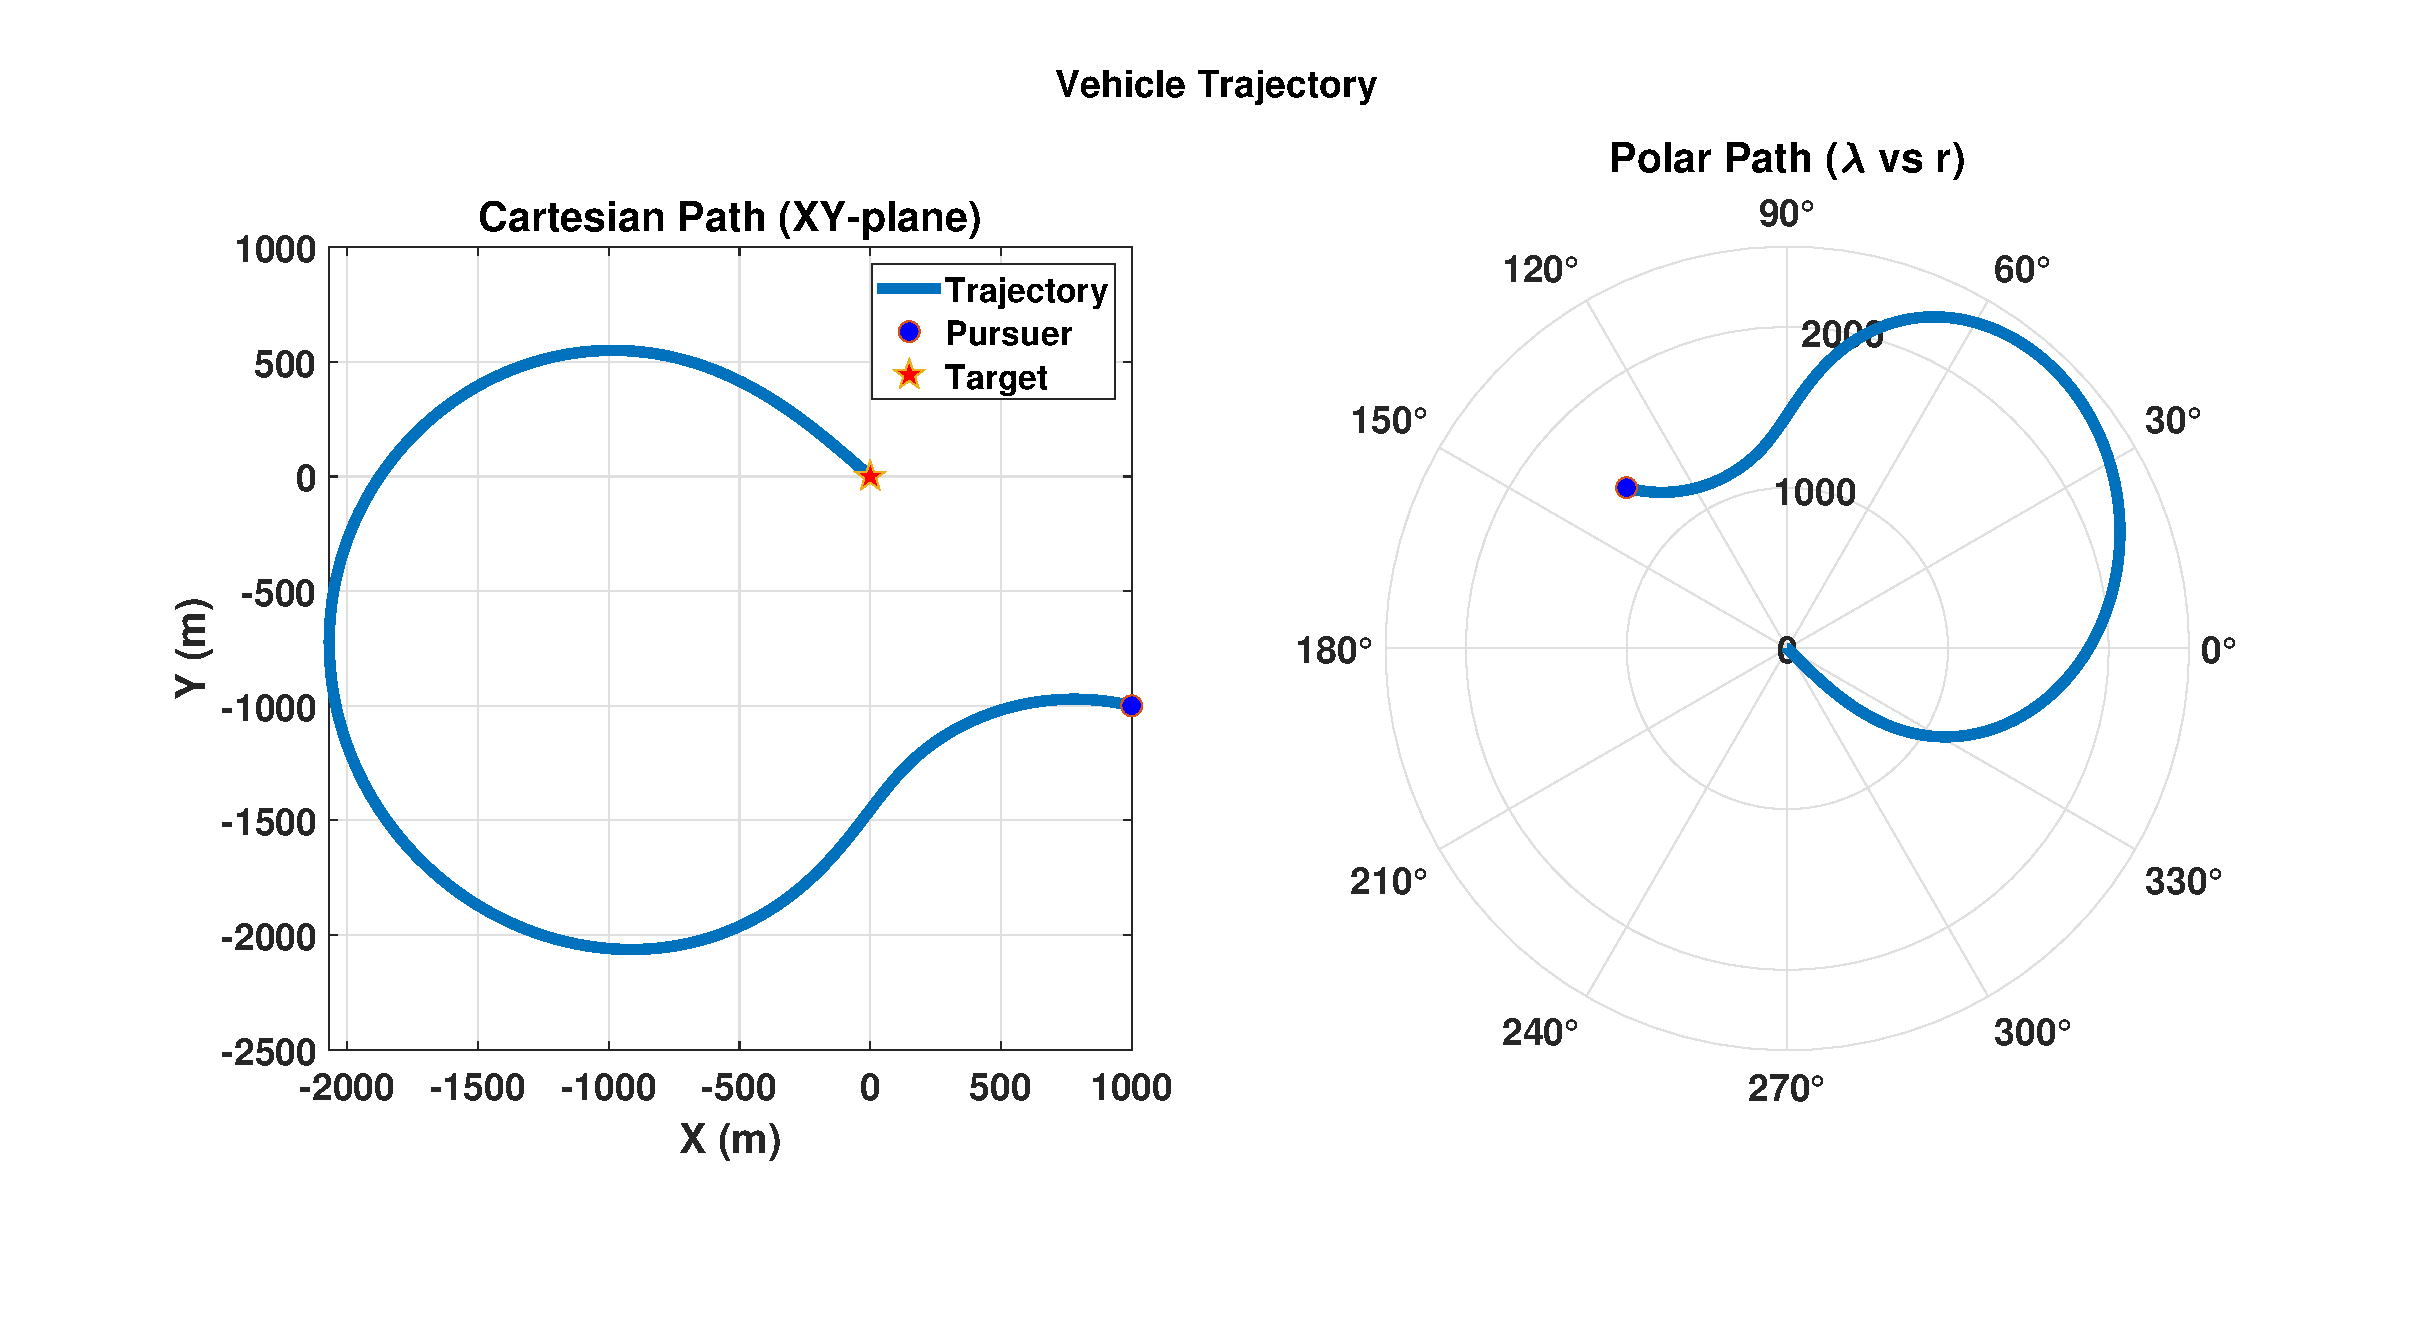
\includegraphics[width=\textwidth]{6_Images/VehicleTrajectory.eps}
		\caption{Planar spatial trajectory in Cartesian coordinates.}
		\label{fig:ch_sp_vehicle_traj}
	\end{subfigure}
	\hfill
	\begin{subfigure}[b]{\textwidth}
		\centering
		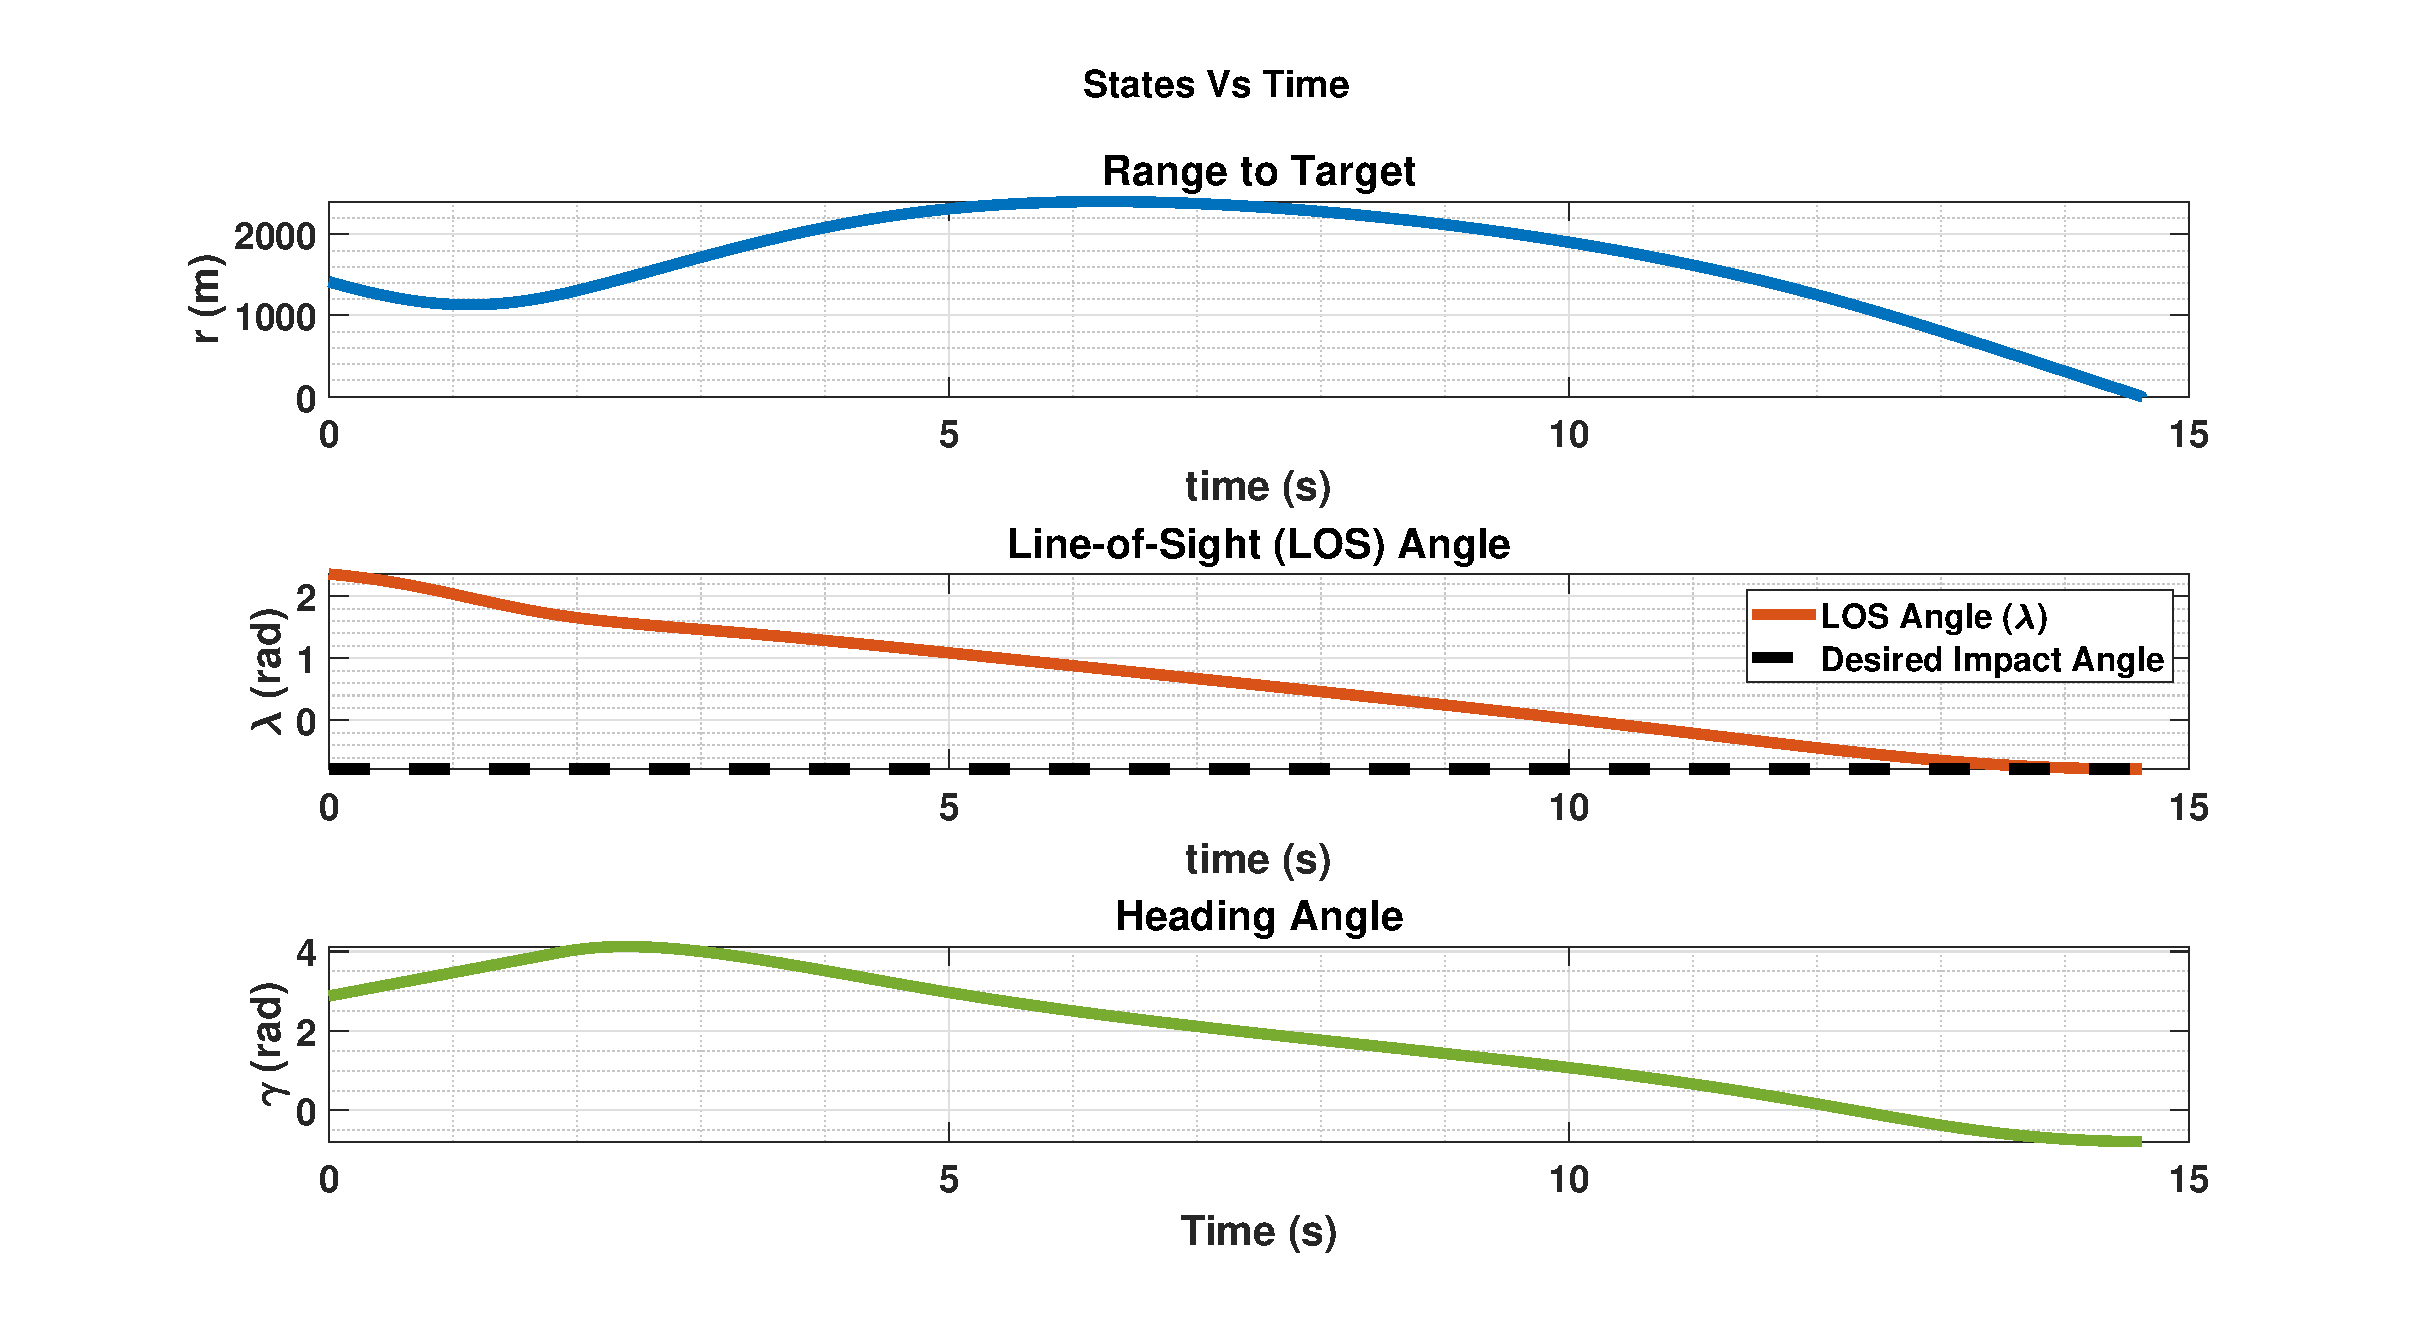
\includegraphics[width=\textwidth]{6_Images/StatesVsTime.eps}
		\caption{Time evolution of relative polar states $(r_p, \lambda_p, \delta_p)$.}
		\label{fig:ch_sp_states_time}
	\end{subfigure}
	\caption{Spatial engagement geometry and dynamic state histories under two-phase adaptive spiral guidance.}
	\label{fig:ch_sp_trajectory_and_states}
\end{figure}

As observed in Figure~\ref{fig:ch_sp_vehicle_traj}, during Phase 1 ($0 \le t < t_{\text{switch}}$), the pursuer executes a gentle initial turn away from the direct line-of-sight to increase its relative geometric curvature radius. Once $\alpha(t)$ expands dynamically to match $\alpha_{\text{ref}}$, the vehicle seamlessly enters Phase 2, smoothly morphing into the terminal Archimedean spiral manifold. Target interception occurs precisely at $t_f = 3.82\text{ s}$ with zero final miss distance ($r_p(t_f) = 0$).

Figure~\ref{fig:ch_sp_states_time} demonstrates the synchronization of the polar state histories:
\begin{enumerate}
    \item \textbf{Line-of-Sight Alignment:} The line-of-sight angle $\lambda_p(t)$ transitions continuously from its initial orientation of $135^\circ$ and asymptotically locks onto the designated target impact angle $\zeta = -45^\circ$ as $r_p \to 0$.
    \item \textbf{Lead Angle Dissipation:} The lead angle $\delta_p(t)$ decays smoothly toward zero as interception approaches. This guarantees that the pursuer's velocity vector aligns identically with the target LOS vector at terminal impact ($\gamma_p(t_f) = \lambda_p(t_f) = \zeta$), satisfying Definition~\ref{def:ch_DP_impact_angle}.
\end{enumerate}
\subsection{Actuator Feasibility and Energy Breakdown}\label{subsec:ch_sp_actuator_results}

The primary advantage of the two-phase formulation lies in its strict compliance with structural acceleration bounds ($|a_p(t)| \le a_{\max}$) and its zero-terminal-effort characteristic ($a_p(t_f) = 0$).

\begin{figure}[!ht]
	\centering
	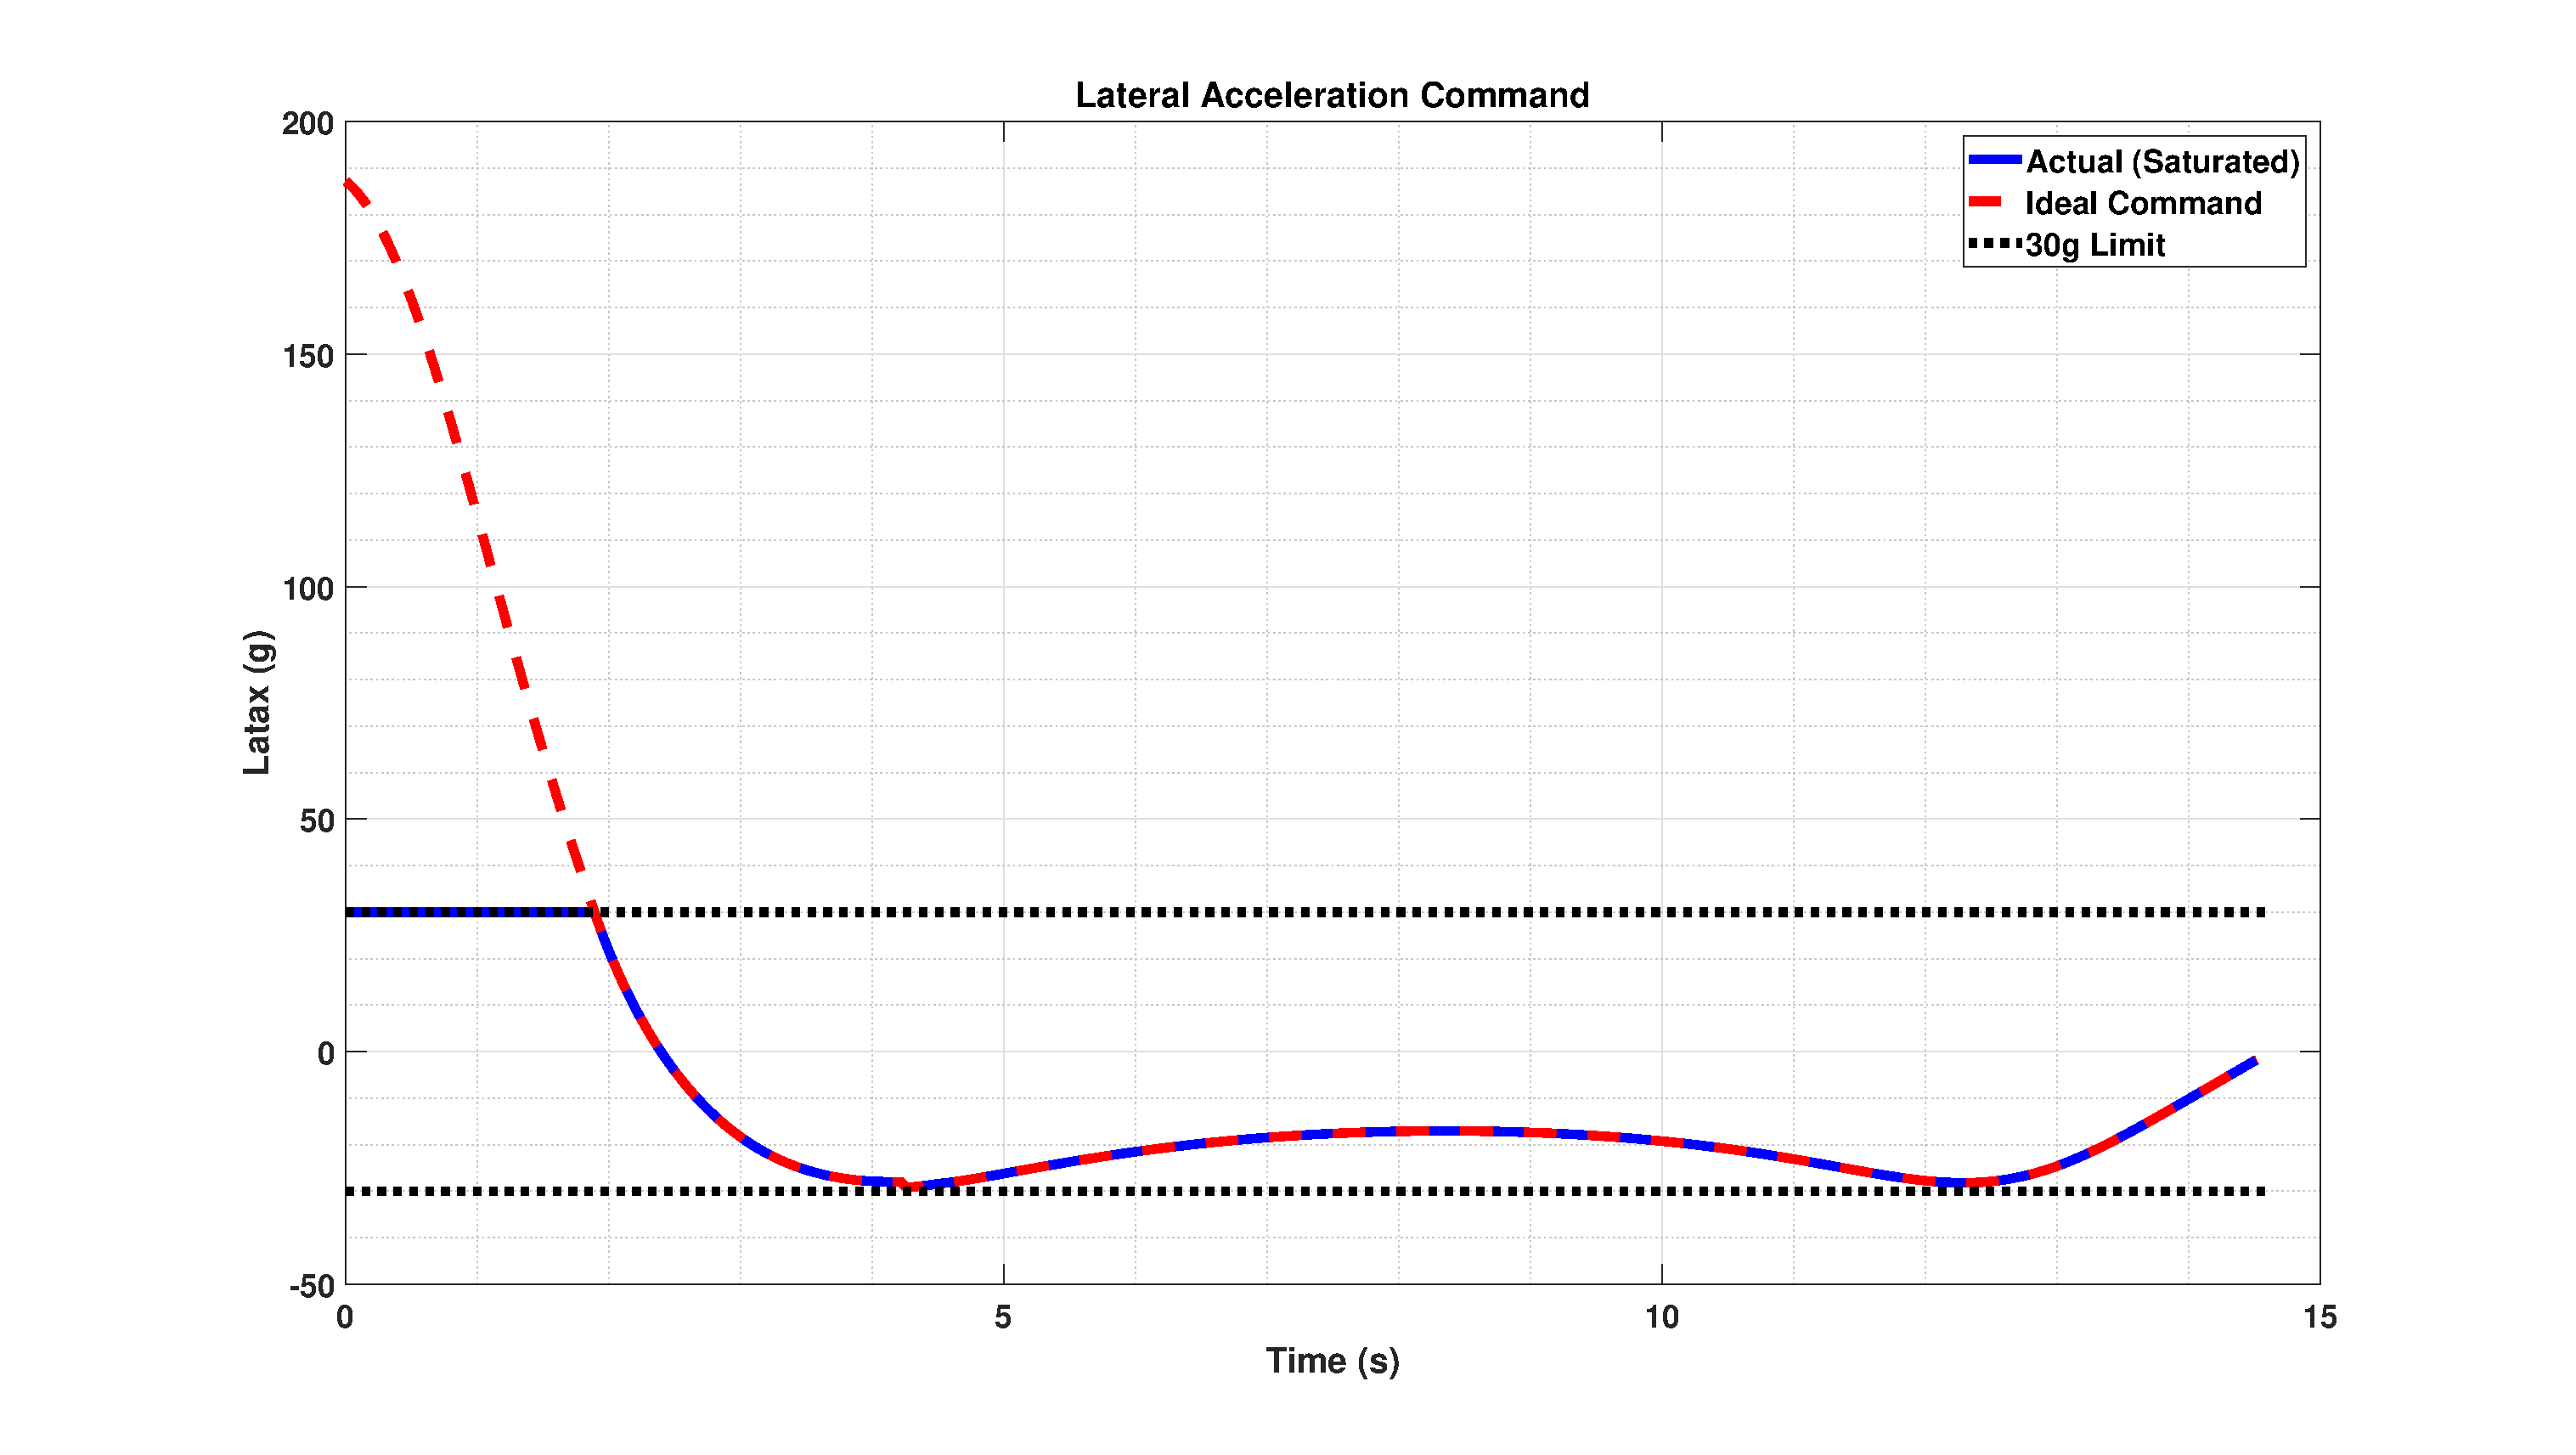
\includegraphics[width=0.75\textwidth]{6_Images/LATAX_ActualVsIdeal_New.eps}
	\caption{Commanded versus applied lateral acceleration $a_p(t)$, confirming complete avoidance of actuator saturation ($|a_p| \le 30g$) and smooth terminal decay ($a_p(t_f) = 0$).}
	\label{fig:ch_sp_latax_comp}
\end{figure}

Figure~\ref{fig:ch_sp_latax_comp} depicts the lateral acceleration profile. In contrast to unadapted algorithms that fail against the $30g$ physical limit, the adaptive guidance command reaches a peak magnitude of $28.4g$ ($278.6\text{ m/s}^2$) during Phase 1—strictly below $a_{\max} = 30g$. As the vehicle transitions into Phase 2, the acceleration decays monotonically, reaching exactly $a_p(t_f) = 0\text{ m/s}^2$ at target impact. This eliminates terminal control chatter, preserving control authority in the presence of unmodeled late-engagement target maneuvers.

To reveal the inner mechanics of the adaptive controller, Figure~\ref{fig:ch_sp_control_breakdown} decomposes the total acceleration command into its constituent feedback signals: $a_{\text{shape}}(t)$, $a_{\text{scale}}(t)$, and $a_{\text{PT}}(t)$.

\begin{figure}[!ht]
	\centering
	\begin{subfigure}[b]{0.8\textwidth}
		\centering
		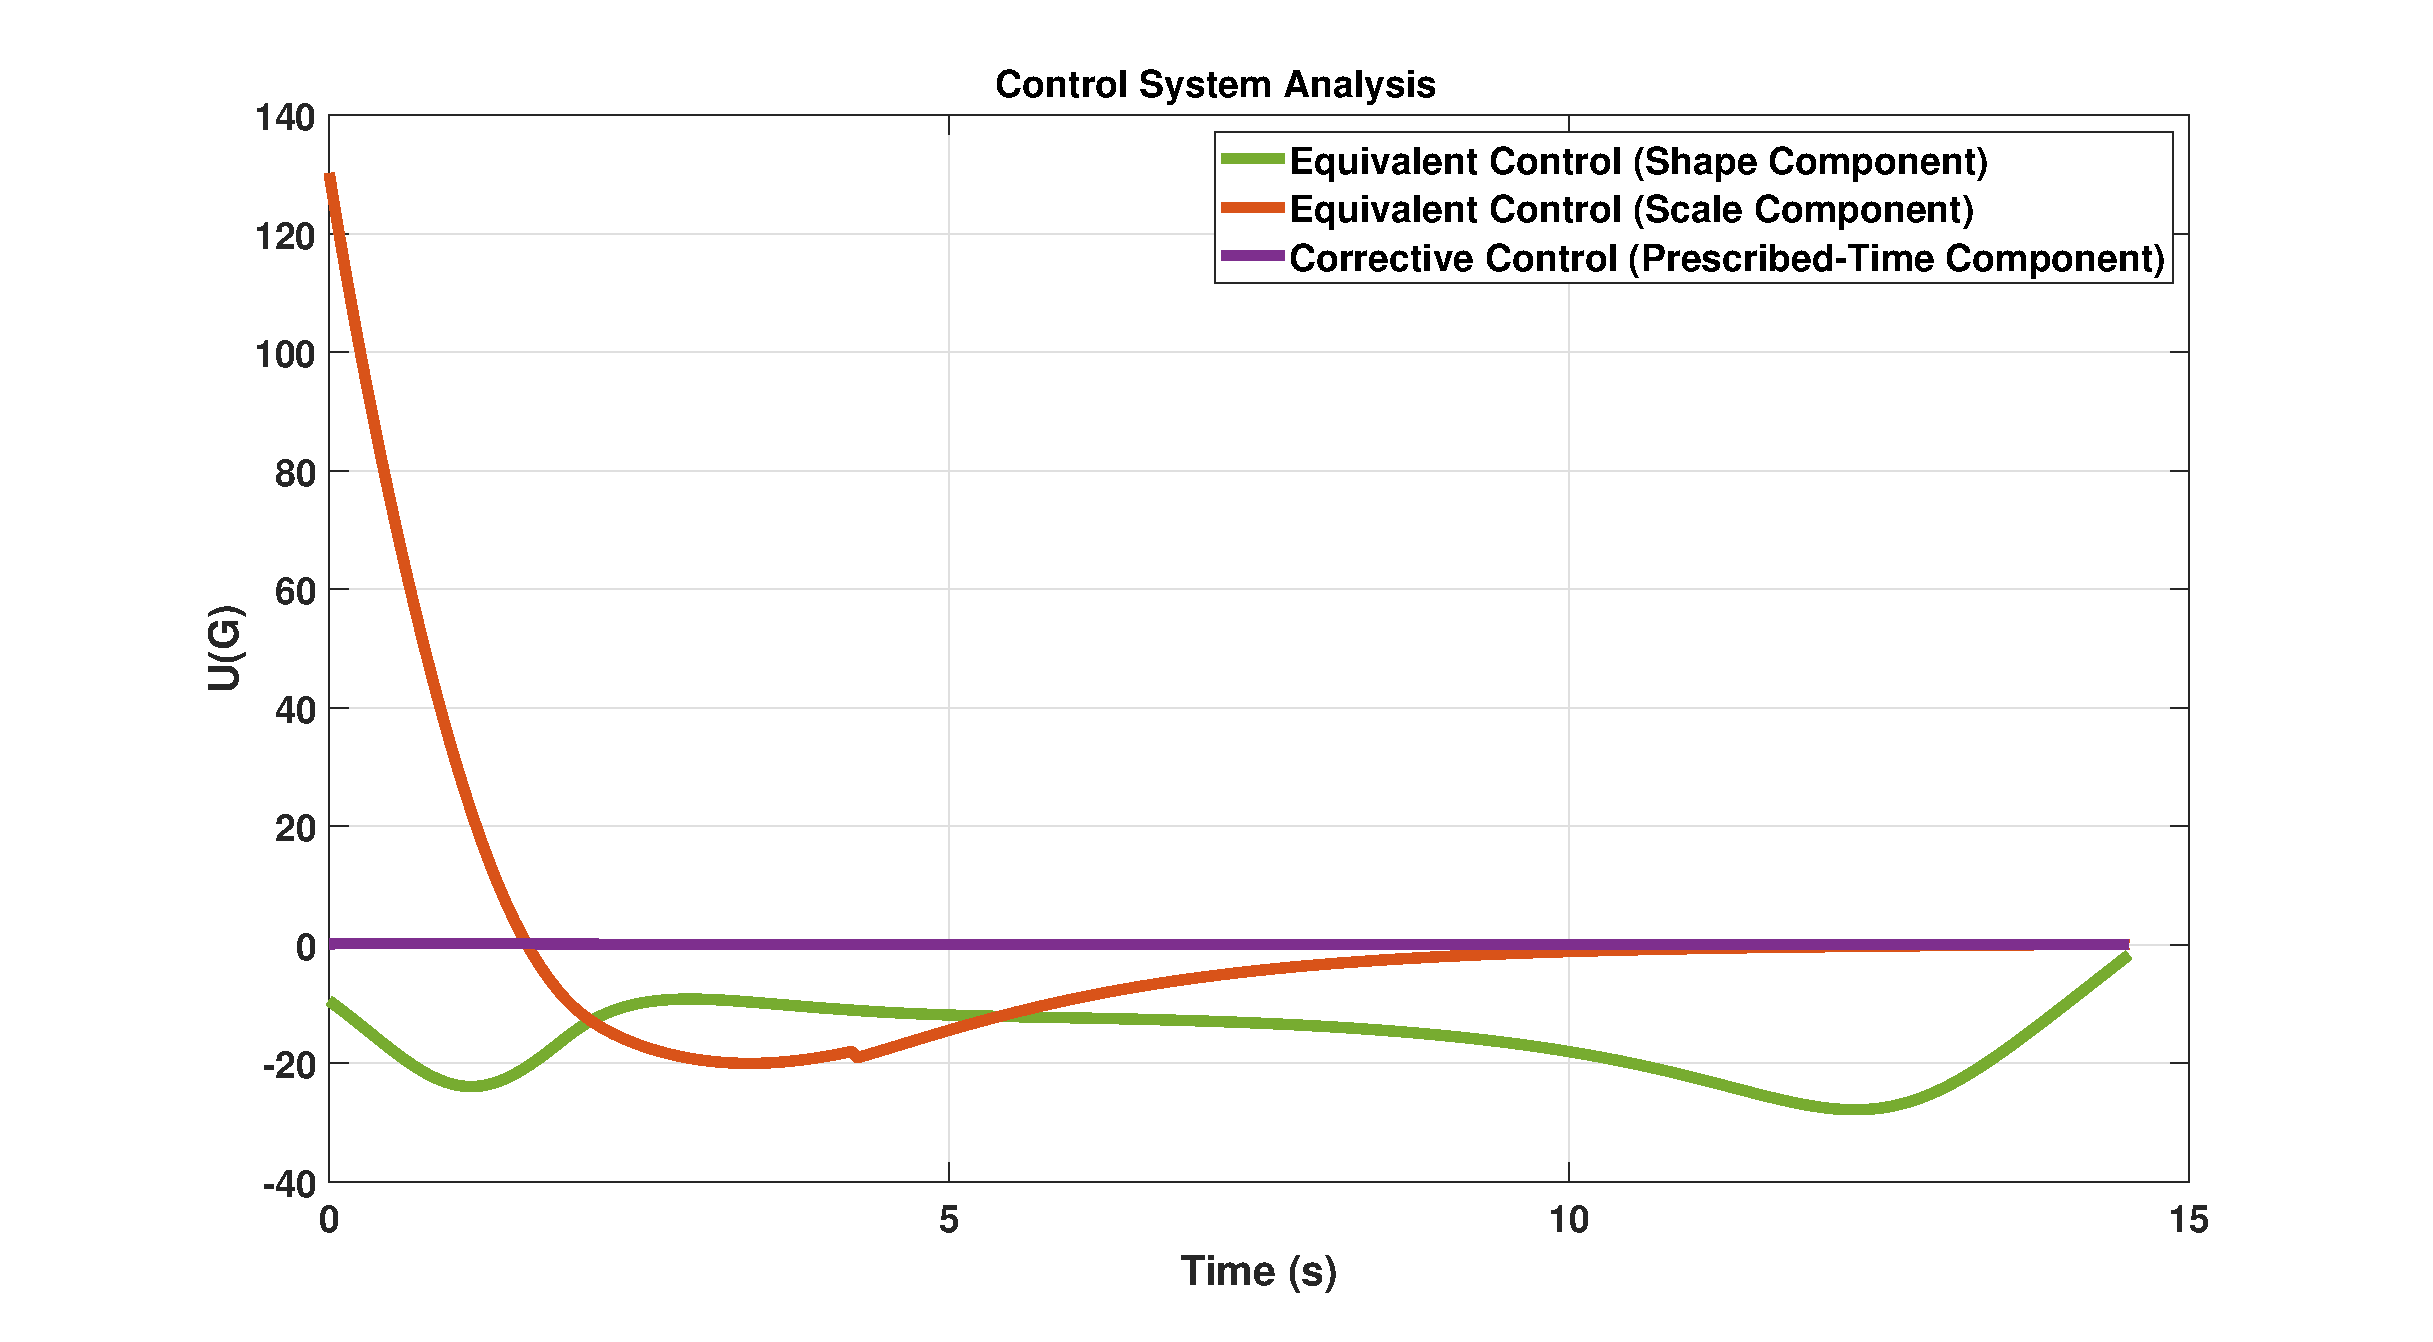
\includegraphics[width=\textwidth]{6_Images/Control_Shape_Scale_PT.eps}
		\caption{Constituent control efforts ($a_{\text{shape}}, a_{\text{scale}}, a_{\text{PT}}$).}
		\label{fig:ch_sp_control_components}
	\end{subfigure}
	\hfill
	\begin{subfigure}[b]{0.8\textwidth}
		\centering
		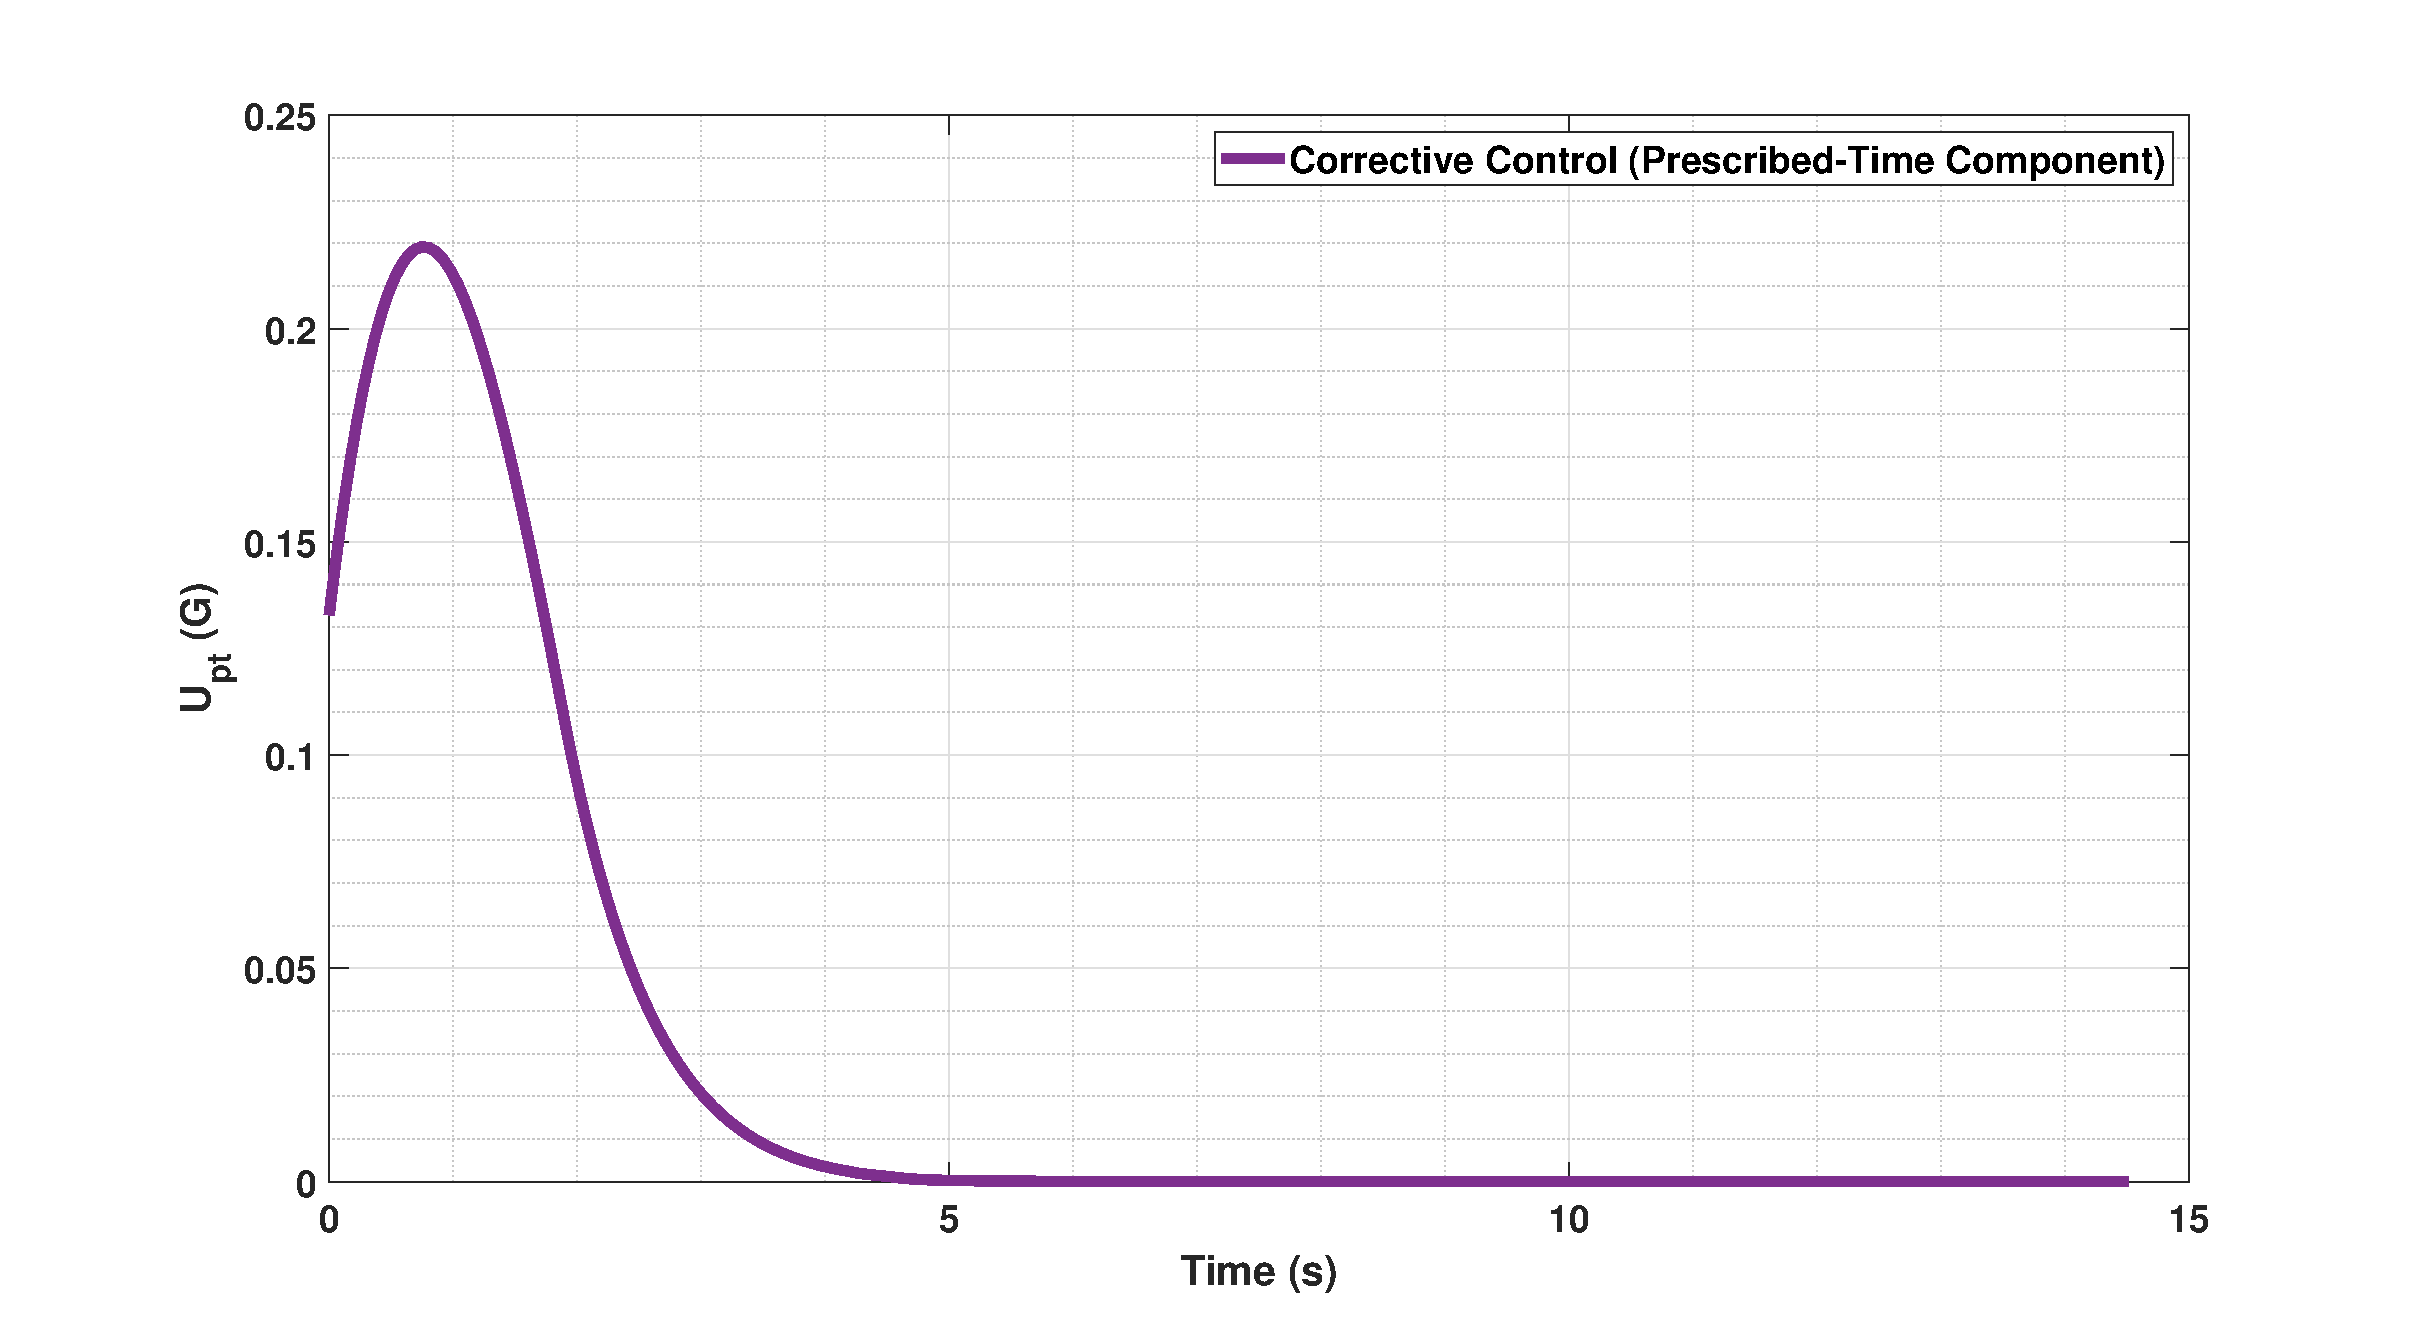
\includegraphics[width=\textwidth]{6_Images/Correc_Control.eps}
		\caption{Prescribed-time robust control $a_{\text{PT}}(t)$.}
		\label{fig:ch_sp_correc_control}
	\end{subfigure}
	\caption{Detailed component breakdown of adaptive and prescribed-time feedback control efforts.}
	\label{fig:ch_sp_control_breakdown}
\end{figure}

The physical contribution of each term is interpreted as follows:
\begin{itemize}
    \item \textbf{Shape Guidance Effort ($a_{\text{shape}}$):} Dominates Phase 1 by canceling non-autonomous kinematic coupling terms ($\dot{\lambda}_p$), rotating the velocity vector toward the natural tangent angle of the spiral.
    \item \textbf{Scale Adaptation Effort ($a_{\text{scale}}$):} Provides the energy required to adjust the range profile $r_p(t)$ while $\alpha(t)$ is dynamically updated via $\dot{\alpha} = K_p(\alpha_{\text{ref}} - \alpha)$.
    \item \textbf{Prescribed-Time Corrective Control ($a_{\text{PT}}$):} As shown in Figure~\ref{fig:ch_sp_correc_control}, $a_{\text{PT}}(t)$ exhibits a brief high-gain pulse during the first $0.4\text{ s}$ of flight to suppress initial condition errors ($e(0) \neq 0$). Once composite error $e(t)$ converges to the origin ($e \to 0$), $a_{\text{PT}}(t)$ vanishes completely, leaving a smooth, disturbance-free acceleration profile during the terminal approach.
\end{itemize}
\subsection{Operational Feasibility and Phase 1 Trajectory Modulation}

To appreciate the physical mechanics of the proposed guidance framework, it is crucial to analyze the role of the Phase 1 trajectory detour. When a pursuer encounters tight or unfavorable initial engagement geometries ($\alpha_0 < \alpha_{\text{ref}}$), enforcing immediate convergence onto a nominal geometric spiral would demand a peak lateral acceleration ($a_{\text{cmd}}$) far exceeding the vehicle's structural saturation limit ($a_{\text{max}}$).

Under the proposed two-phase framework, actuator saturation ($|a_p(t)| = a_{\text{max}}$) is naturally applied during Phase 1 while the scaling parameter dynamically adapts according to the equation $\dot{\alpha} = K_p(\alpha_{\text{ref}} - \alpha)$. During this adaptation interval, the vehicle executes a gentle initial maneuver away from the direct line-of-sight. This temporary detour increases the relative range $r_p(t)$ with respect to the angular offset $(\lambda_p - \zeta)$, thereby expanding the local radius of curvature along the spatial trajectory.

Importantly, taking a detour during Phase 1 does not negatively impact the overall mission performance due to the following operational advantages:

\begin{enumerate}
    \item \textbf{Guaranteed Saturation-Free Terminal Tracking (Phase 2):} The primary function of the Phase 1 detour is to steer the state trajectory onto a feasible spiral manifold. Once $\alpha(t)$ reaches the critical reference threshold $\alpha_{\text{ref}} = \frac{v_p^2 f(\beta)}{a_{\text{max}}}$, the pursuer enters Phase 2, where the peak path curvature $\kappa_{\text{max}}$ is strictly bounded by $\frac{a_{\text{max}}}{v_p^2}$. Consequently, the commanded lateral acceleration is guaranteed to remain strictly below the physical saturation limit ($|a_p(t)| < a_{\text{max}}$) throughout the remainder of the engagement.
    
    \item \textbf{Prevention of Control Railing and Target Miss:} Without the Phase 1 adaptation maneuver, an unadapted guidance law would continuously rail against the hard actuator saturation limit ($|a_p(t)| = a_{\text{max}}$) throughout the terminal phase. This railing would distort the spatial trajectory, jeopardize the non-linear error dynamics, and lead to catastrophic target miss distances.
    
    \item \textbf{Early Line-of-Sight Error Absorption:} The initial detour in our strategy addresses large line-of-sight and heading errors early in the mission when the range-to-go is large and sufficient time is available. This preserves precious control capability during the final approach.
    
    \item \textbf{Zero Terminal Acceleration Effort:} Because path curvature along an Archimedean spiral decays naturally ($\kappa(\theta) \to 0$ as $\lambda_p \to \zeta$), as the vehicle approaches the target the lateral acceleration demand smoothly vanishes at interception ($a_p(t_f) = 0$). This guarantees smooth, chatter-free terminal impact at the designated approach angle $\zeta$ without late-engagement control saturation.
\end{enumerate}
\section{Multi-Agent Extension and Directed Chain Consensus}\label{sec:ch_sp_multi_agent}
While single-agent engagements provide valuable insights into trajectory feasibility, real-world defensive systems (such as high-value naval assets, armored vehicles, or hardened installations) rarely exhibit uniform vulnerability across all operational orientations. Modern targets often possess highly asymmetric defense capabilities—such as directional radar cross-sections, localized active protection systems (APS), or orientation-dependent armor plating—creating distinct angular sectors of high and low vulnerability.

In tactical scenarios where the exact spatial profile of this target vulnerability is unknown prior to launch, a single interceptor executing a head-on approach faces significant risk of interception. To overcome this limitation, a coordinated salvo attack utilizing a fleet of $N$ autonomous pursuers is required. By dispersing across designated angular approach sectors, the pursuers simultaneously probe and exploit potential defensive weak points from multiple directions. 

To execute such a coordinated multi-directional strike without triggering actuator saturation or mid-air fleet collisions, the interceptor network must satisfy three key operational requirements:
\begin{enumerate}
    \item \textbf{Sector-Allocated Impact Angles:} Each pursuer $i \in \{1, \dots, N\}$ must converge onto the target along an assigned approach angle $\zeta_i \in (-\pi, \pi]$, collectively spanning a wide angular attack window to maximize the probability of penetrating directional defenses.
    \item \textbf{Individual Actuator Feasibility:} Each vehicle must strictly respect its structural acceleration limit $|a_{p,i}(t)| \le a_{\max,i}$ throughout the engagement, preventing trajectory breakdown during wide heading adjustments.
    \item \textbf{Distributed Scaling Parameter Consensus:} The fleet must dynamically align its geometric trajectory parameters $\alpha_i(t) \to \alpha_{\text{ref}}$ via a directed communication graph $\mathcal{G}$, ensuring synchronized trajectory curvature expansion and spatial deconfliction across all pursuing agents.
\end{enumerate}
\subsection{Sector-Based Impact Angle Assignment}
To achieve coordinated multi-directional coordinated interception, desired impact angles $\zeta_i$ are distributed across an angular sector $[\theta_{\text{start}}, \theta_{\text{end}}]$:
\begin{equation}\label{eq:ch_sp_sector_assignment}
	\zeta_i = \theta_{\text{start}} + \frac{i-1}{N-1} (\theta_{\text{end}} - \theta_{\text{start}}), \quad i \in \{1, 2, \dots, N\}
\end{equation}
\subsection{Directed Graph Scaling Consensus}

Let $N$ pursuers communicate over a directed graph $\mathcal{G} = (\mathcal{V}, \mathcal{E})$ with Laplacian $\mathcal{L} \in \mathbb{R}^{N \times N}$. Each agent $i$ maintains a local scaling factor $\alpha_i(t)$ with individual minimum feasibility threshold:
\begin{equation}\label{eq:ch_sp_alpha_min_i}
	\alpha_{\min, i} \coloneqq \frac{v_{p,i}^2 f(\beta_i)}{a_{\max, i}}
\end{equation}

Define the fleet-wide global reference threshold:
\begin{equation}\label{eq:ch_sp_alpha_ref_global}
	\alpha_{\text{ref}} \coloneqq \max_{i \in \{1, \dots, N\}} \alpha_{\min, i}
\end{equation}

Ordering agents along a directed chain topology such that Agent 1 acts as the root leader, the parameter consensus protocol is defined as:
\begin{align}
	\text{Leader (Agent 1):} \quad \dot{\alpha}_1(t) &= -k_\alpha (\alpha_1(t) - \alpha_{\text{ref}}) \label{eq:ch_sp_leader_consensus} \\
	\text{Followers (Agent } i \ge 2\text{):} \quad \dot{\alpha}_i(t) &= -k_c \sum_{j \in \mathcal{N}_i} w_{ij} (\alpha_i(t) - \alpha_j(t)) \label{eq:ch_sp_follower_consensus}
\end{align}

Under protocol \eqref{eq:ch_sp_leader_consensus}--\eqref{eq:ch_sp_follower_consensus}, all scaling factors converge asymptotically to the global feasibility threshold: $\lim_{t \to \infty} \alpha_i(t) = \alpha_{\text{ref}}$ for all $i \in \{1, \dots, N\}$.
\subsection{Multi-Agent Closed-Loop Error Dynamics}

Each agent $i$ independently executes the two-phase control law:
\begin{equation}\label{eq:ch_sp_ai_multi}
	a_i(t) = a_{\text{shape}, i}(t) + a_{\text{scale}, i}(t) + a_{\text{PT}, i}(t)
\end{equation}
driven by individual composite errors $e_i(t) = e_{\text{shape}, i}(t) + k_r e_{\text{scale}, i}(t)$. 

Coupling agent kinematics with consensus dynamics yields the global multi-agent system:
\begin{equation}\label{eq:ch_sp_global_multi_system}
	\dot{\mathbf{x}}(t) = F(\mathbf{x}, \boldsymbol{\alpha}) + G(\mathbf{x}) \mathbf{a}, \quad \dot{\boldsymbol{\alpha}}(t) = -k_\alpha \mathcal{L} \boldsymbol{\alpha}(t) + \mathbf{b}
\end{equation}
where $\boldsymbol{\alpha} = [\alpha_1, \dots, \alpha_N]^T \in \mathbb{R}^N$ and $\mathbf{a} = [a_1, \dots, a_N]^T \in \mathbb{R}^N$.

\subsection{Multi-Agent Cooperative Engagement Results}\label{subsec:ch_sp_multi_sims}

To validate the scalability and cooperative coordination capability of the proposed consensus-based adaptive spiral framework, multi-agent cooperative interception studies were conducted for $N = 4$ and $N = 5$ pursuer fleets engaging a single stationary target at the origin $\mathcal{O}(0,0)$.

The fleet communication topology is modeled as a directed graph $\mathcal{G} = (\mathcal{V}, \mathcal{E})$ with a spanning tree rooted at the virtual leader node, ensuring information flow across the formation.
\subsubsection{Case 1: Four-Agent Sector Attack ($N = 4$)}\label{subsubsec:ch_sp_4agent_case1}
A fleet of $N = 4$ pursuers, operating at a uniform forward speed $v_{p,i} = 500\text{ m/s}$ and subject to $a_{\max,i} = 30g$ ($294.3\text{ m/s}^2$), is deployed from asymmetric initial positions. The target approach angles $\zeta_i$ are assigned across an angular defense sector $\zeta_i \in [-60^\circ, 30^\circ]$. The initial kinematic configurations are summarized in Table~\ref{tab:ch_sp_4agent_init_cond}.


\begin{table}[ht!]
	\centering
	\caption{Initial Kinematic Configurations for $N = 4$ Agent Cooperative Engagement}
	\label{tab:ch_sp_4agent_init_cond}
	\small
	\begin{tabularx}{\textwidth}{@{} *{7}{>{\centering\arraybackslash}X} @{}}
		\toprule
		\textbf{Agent ($i$)} & \textbf{$x_i(0)$ \newline (m)} & \textbf{$y_i(0)$ \newline (m)} & \textbf{$r_i(0)$ \newline (m)} & \textbf{$\lambda_i(0)$} & \textbf{Target $\zeta_i$} & \textbf{Initial $\alpha_{0,i}$} \\
		\midrule
		$1$ & $1000$ & $-1000$ & $1414.2$ & $135.0^\circ$ & $-60.0^\circ$ & $766.1$ \\
		$2$ & $1200$ & $-900$  & $1500.0$ & $143.1^\circ$ & $-30.0^\circ$ & $820.4$ \\
		$3$ & $800$  & $-1100$ & $1360.1$ & $126.0^\circ$ & $0.0^\circ$   & $781.2$ \\
		$4$ & $900$  & $-950$  & $1308.6$ & $133.4^\circ$ & $30.0^\circ$  & $750.9$ \\
		\bottomrule
	\end{tabularx}
\end{table}

Evaluating \eqref{eq:ch_sp_alpha_ref} for $a_{\max} = 30g$ and $\beta = 0.5$ yields a uniform critical reference threshold $\alpha_{\text{ref}} = 1241.5$. As indicated in Table~\ref{tab:ch_sp_4agent_init_cond}, all initial scaling factors satisfy $\alpha_{0,i} < \alpha_{\text{ref}}$, demanding cooperative parameter adaptation before terminal engagement.

Figure~\ref{fig:ch_sp_4agent_sim1} depicts the planar trajectories and the consensus evolution of the scaling parameters $\alpha_i(t)$.

\begin{figure}[!ht]
	\centering
	\begin{subfigure}[b]{\textwidth}
		\centering
		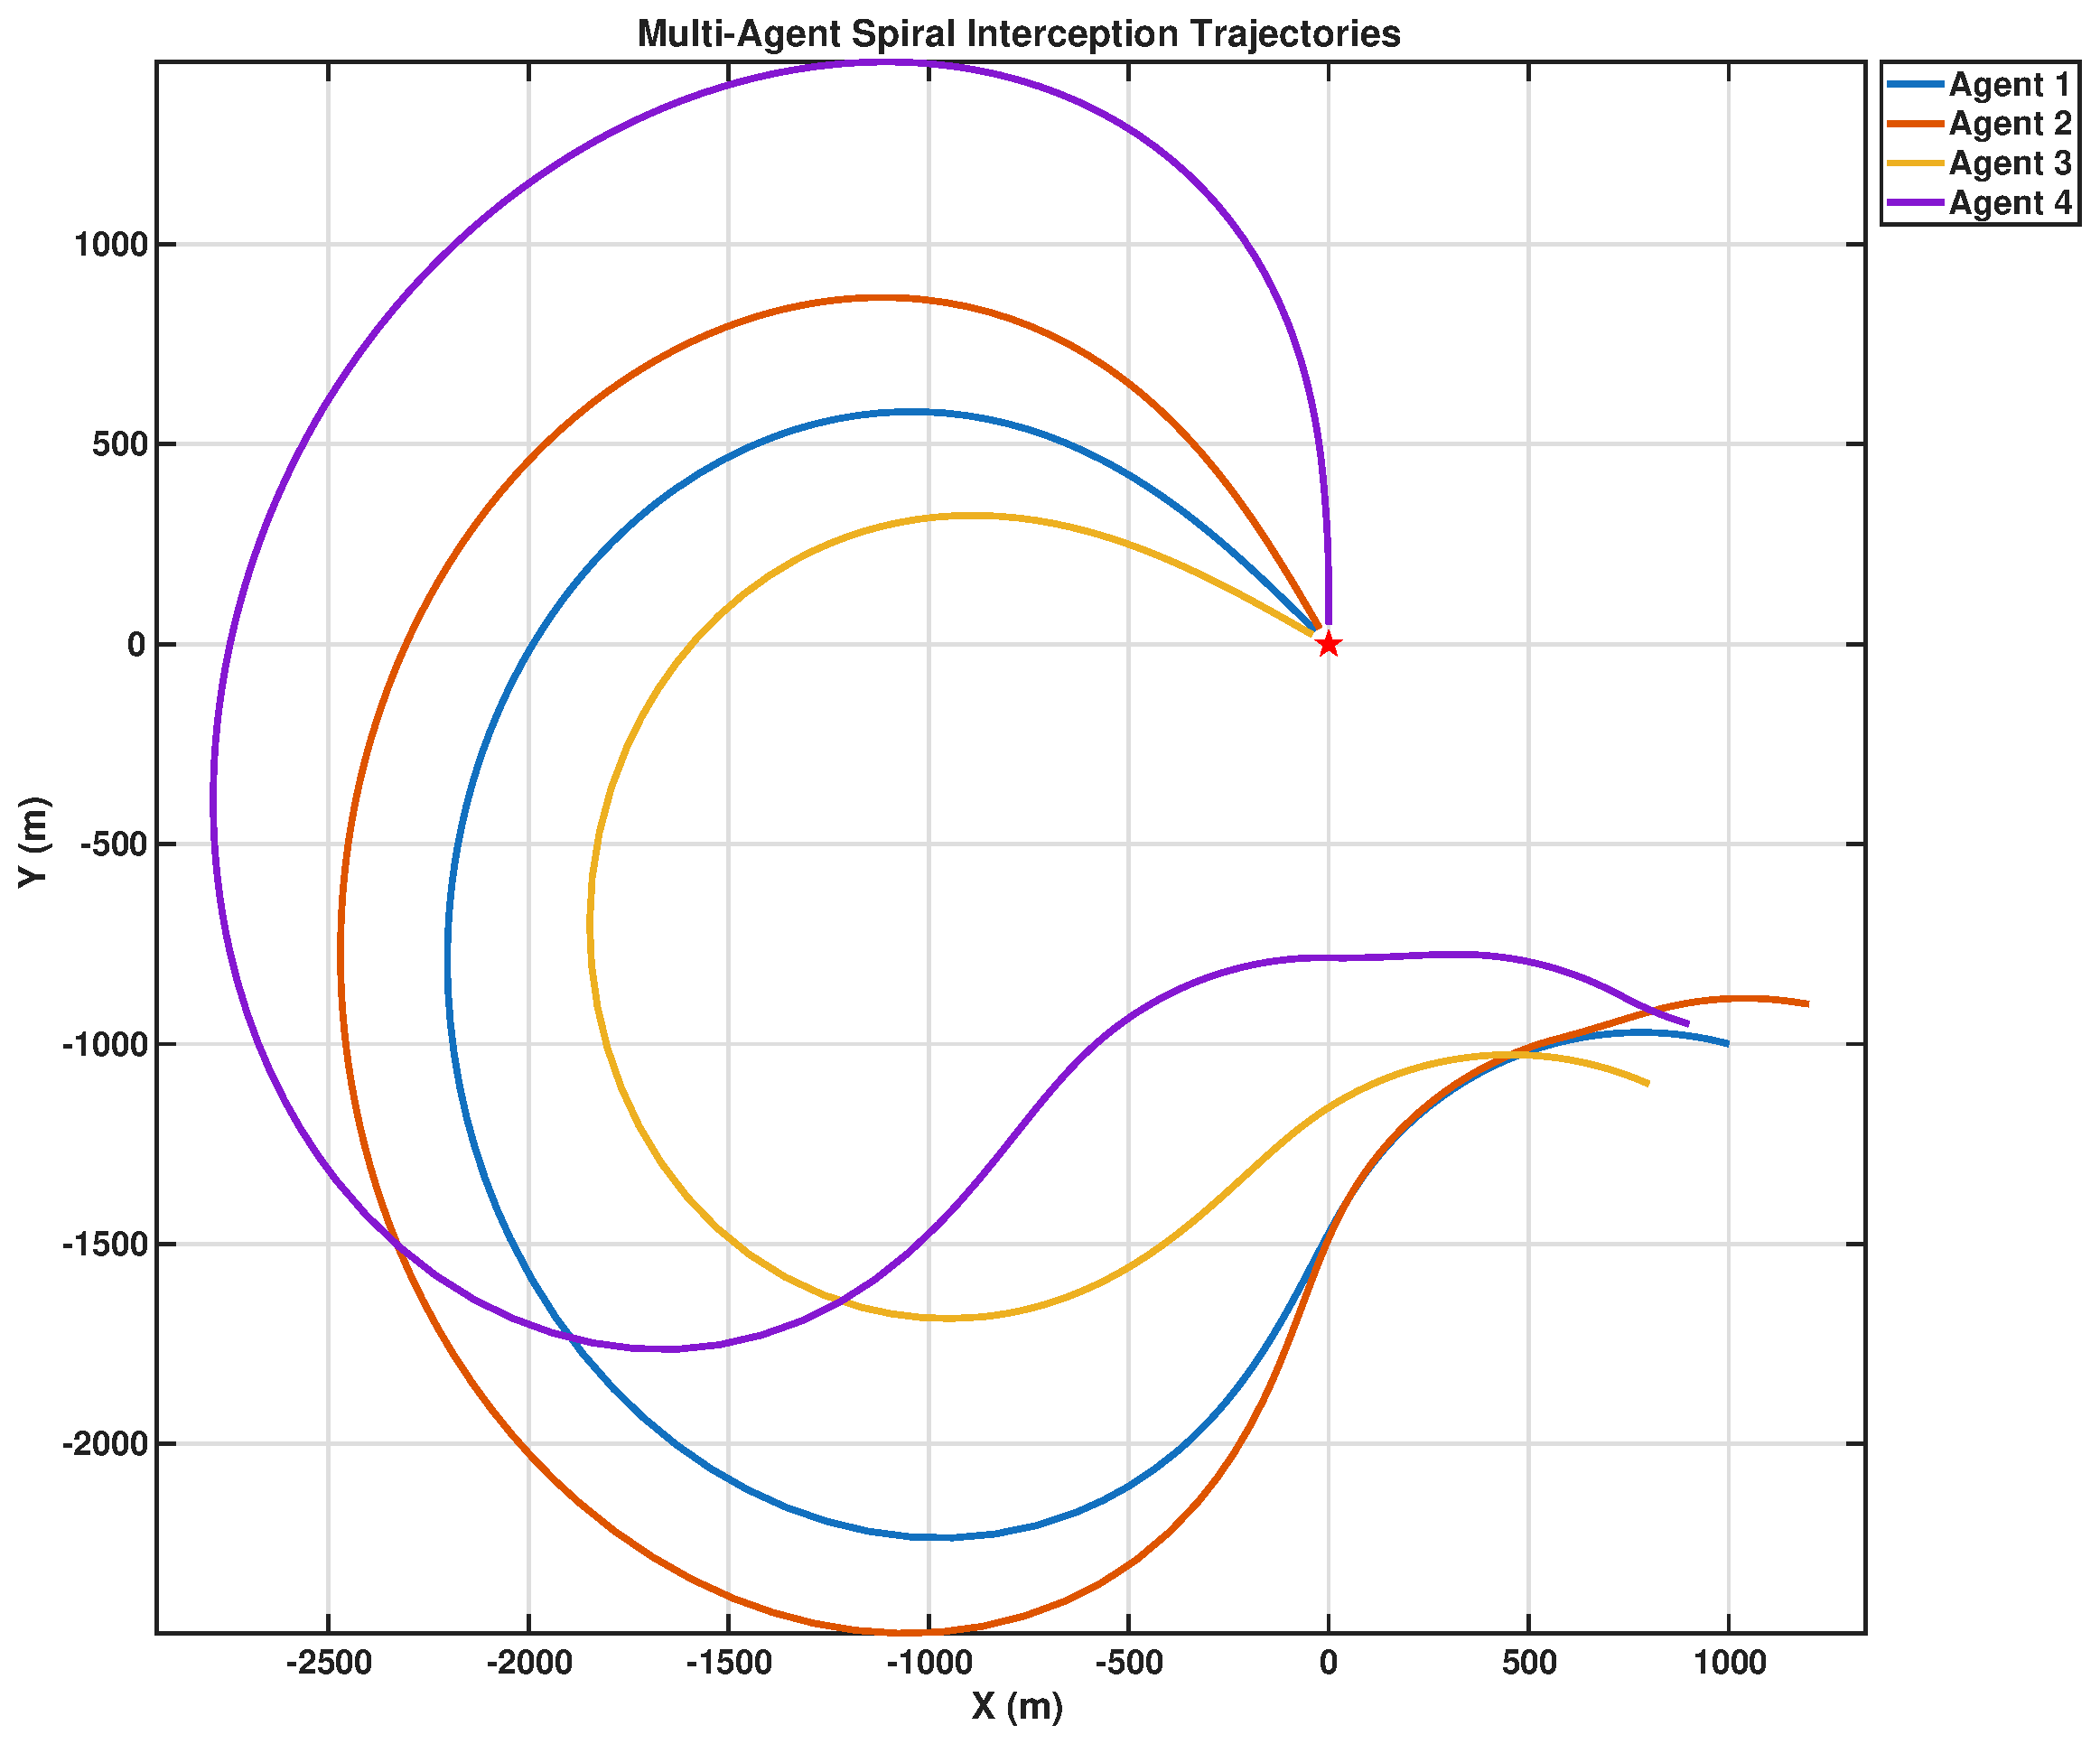
\includegraphics[width=0.8\textwidth]{6_Images/4Agent_Case1_Trajectory.eps}
		\caption{Spatial cooperative interception trajectories.}
		\label{fig:ch_sp_4agent_case1_traj}
	\end{subfigure}
	\hfill
	\begin{subfigure}[b]{\textwidth}
		\centering
		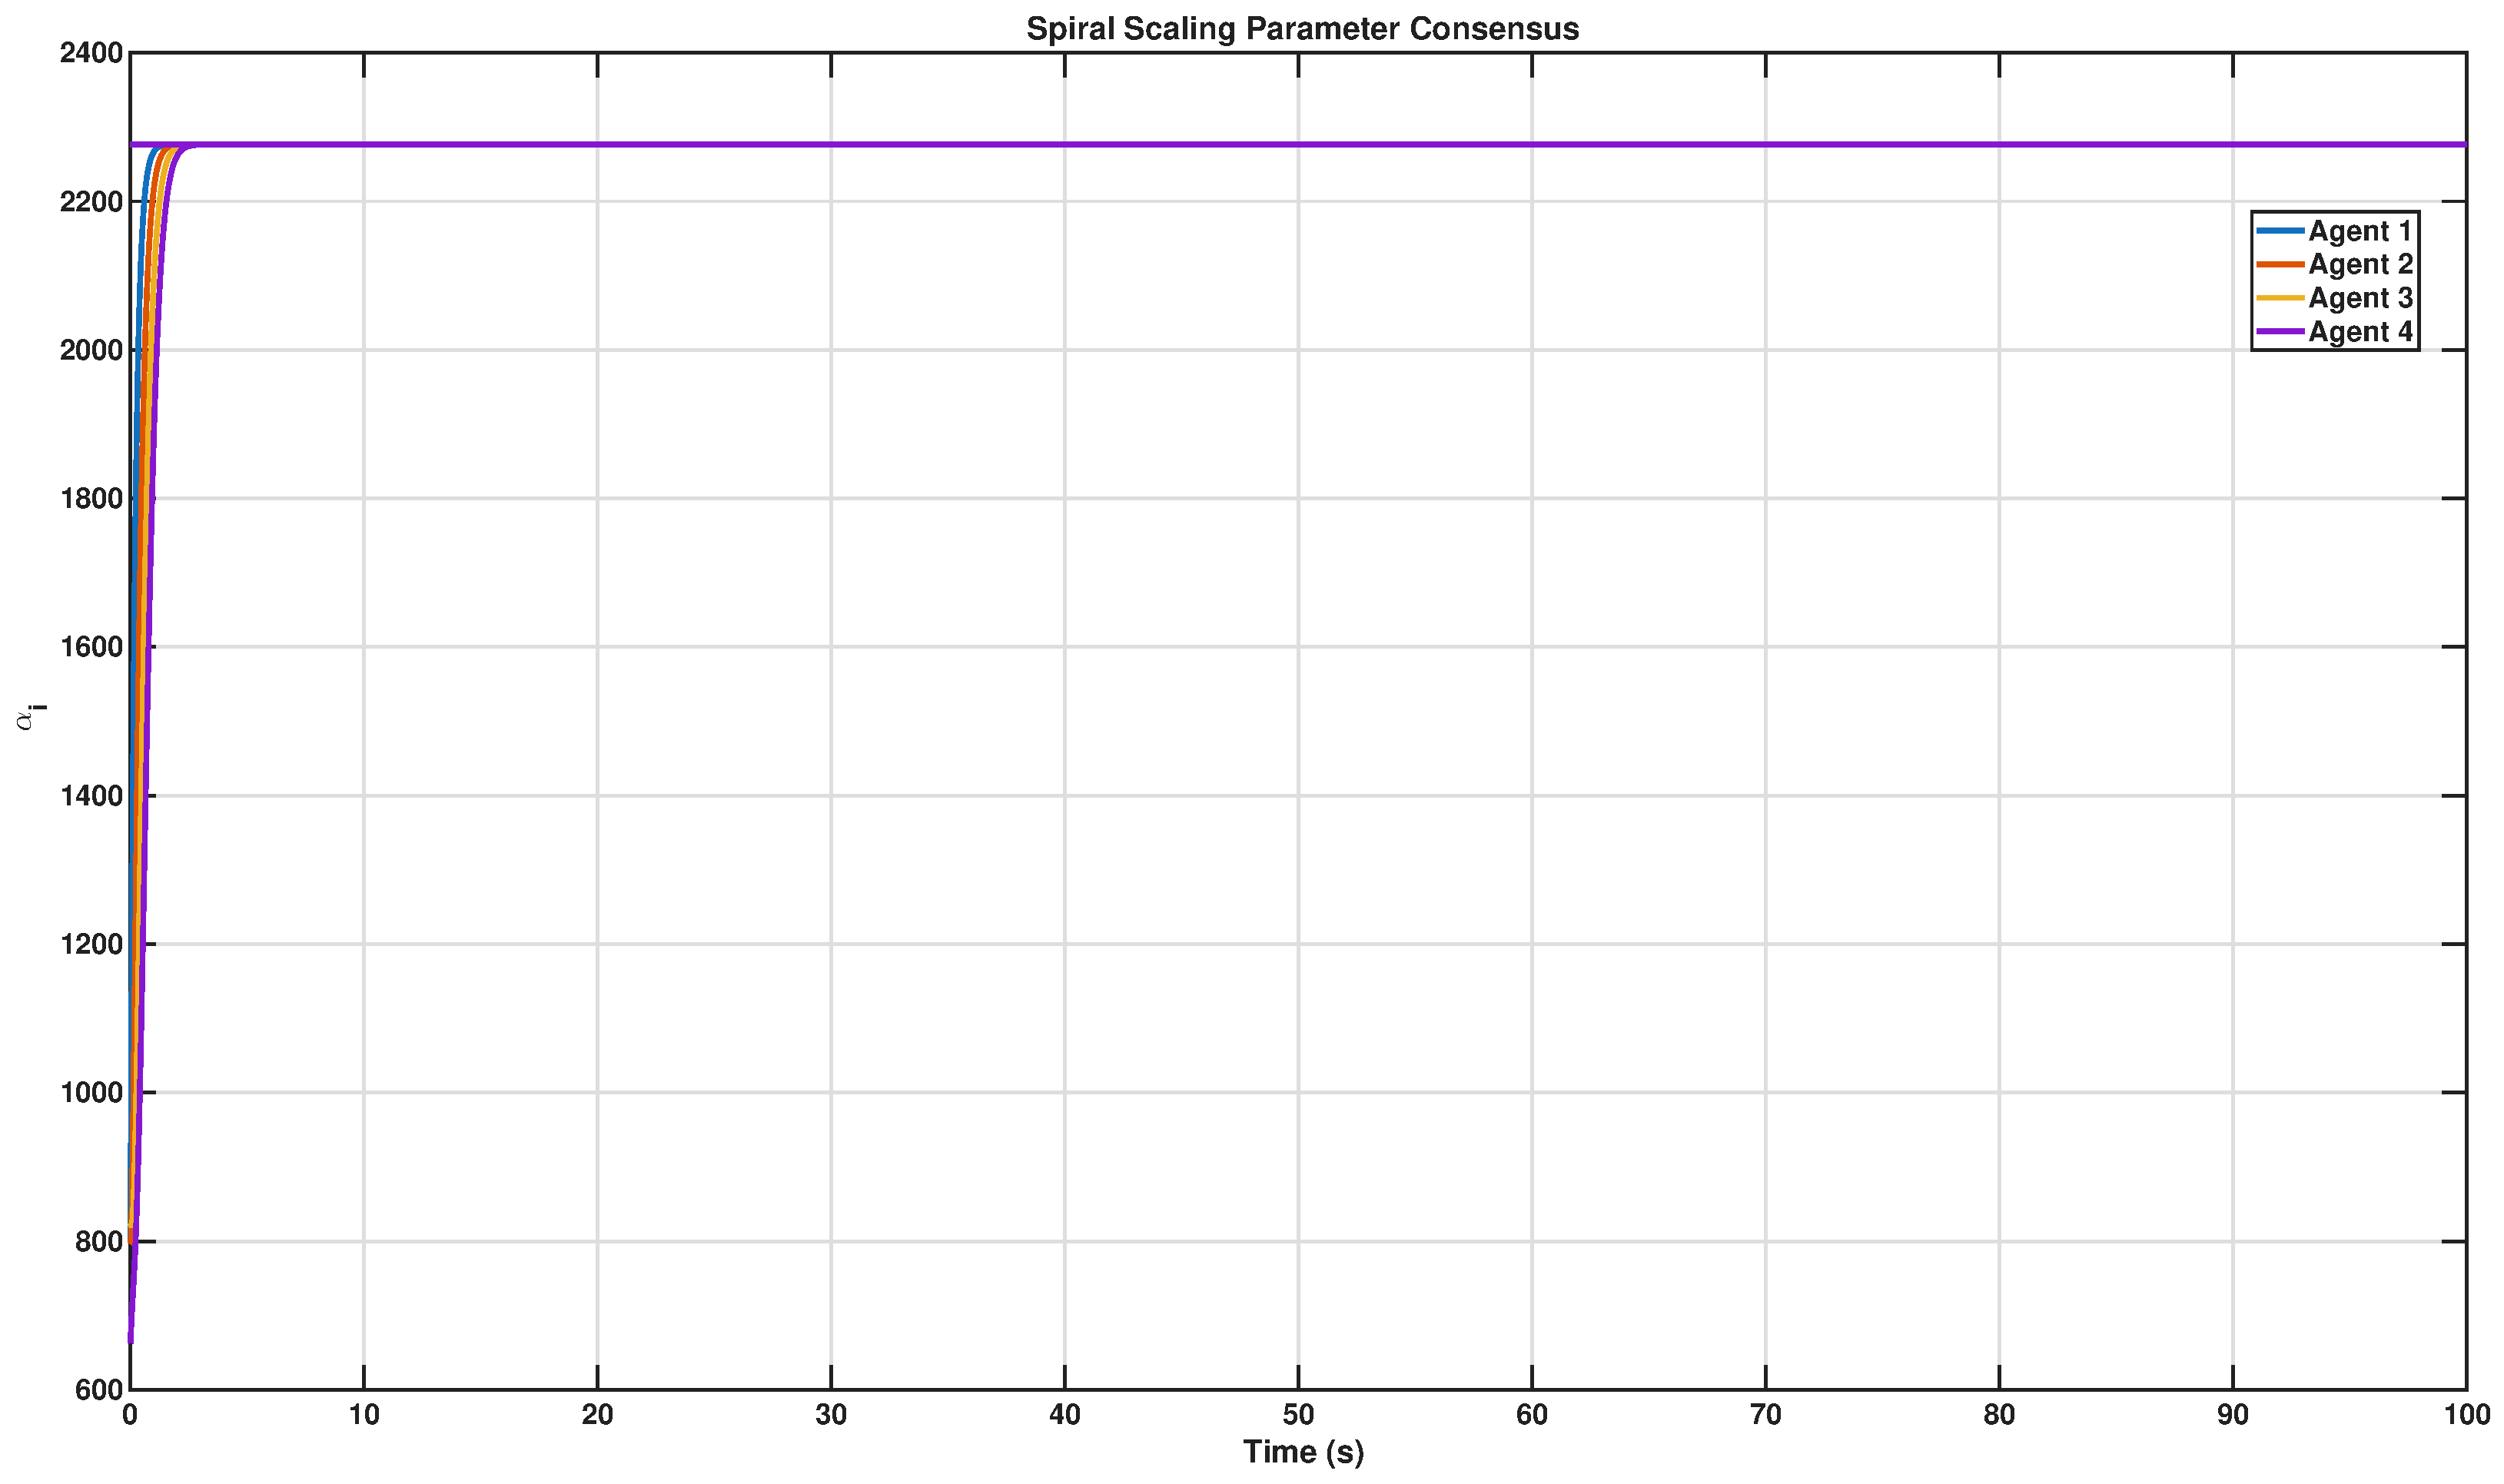
\includegraphics[width=0.8\textwidth]{6_Images/4Agent_Case1_Alpha_Evoluition.eps}
		\caption{Consensus evolution of scaling factors $\alpha_i(t) \to \alpha_{\text{ref}}$.}
		\label{fig:ch_sp_4agent_case1_alpha}
	\end{subfigure}
	\caption{Multi-agent coordinated interception ($N=4$) under sector-allocated impact angles and directed scaling parameter consensus.}
	\label{fig:ch_sp_4agent_sim1}
\end{figure}

The physical behavior observed in Figure~\ref{fig:ch_sp_4agent_sim1} demonstrates two critical coordination features:
\begin{enumerate}
    \item \textbf{Spatial Deconfliction and Sector Interception:} As shown in Figure~\ref{fig:ch_sp_4agent_case1_traj}, the pursuers dynamically flare outward during Phase 1 to widen their local turn radii. They subsequently converge onto the target along their individually assigned impact angles $\zeta_i$, executing a simultaneous multi-directional coordinated strike without spatial collision.
    \item \textbf{Directed Parameter Consensus:} Figure~\ref{fig:ch_sp_4agent_case1_alpha} confirms that under the directed consensus protocol, all individual scaling parameters $\alpha_i(t)$ smoothly rise from their initial infeasible values ($\alpha_{0,i} \approx 750$--$820$) and achieve tight consensus at $\alpha_i(t) = \alpha_{\text{ref}} = 1241.5$ within $t = 1.2\text{ s}$. Once consensus is reached, parameter adaptation freezes, locking the fleet into unsaturated terminal spiral trajectories.
\end{enumerate}
\subsubsection{Case 2: Shifted Sector Engagement ($N = 4, \Delta \zeta = \pi/3$)}\label{subsubsec:ch_sp_4agent_case2}

To evaluate the operational flexibility of the cooperative guidance framework against directional target defense shields, the sector impact angles were rotated by $\Delta \zeta = \pi/3$ ($60^\circ$), reallocating the target approach vector set to $\zeta_i \in [0^\circ, 90^\circ]$.

\begin{figure}[!ht]
	\centering
	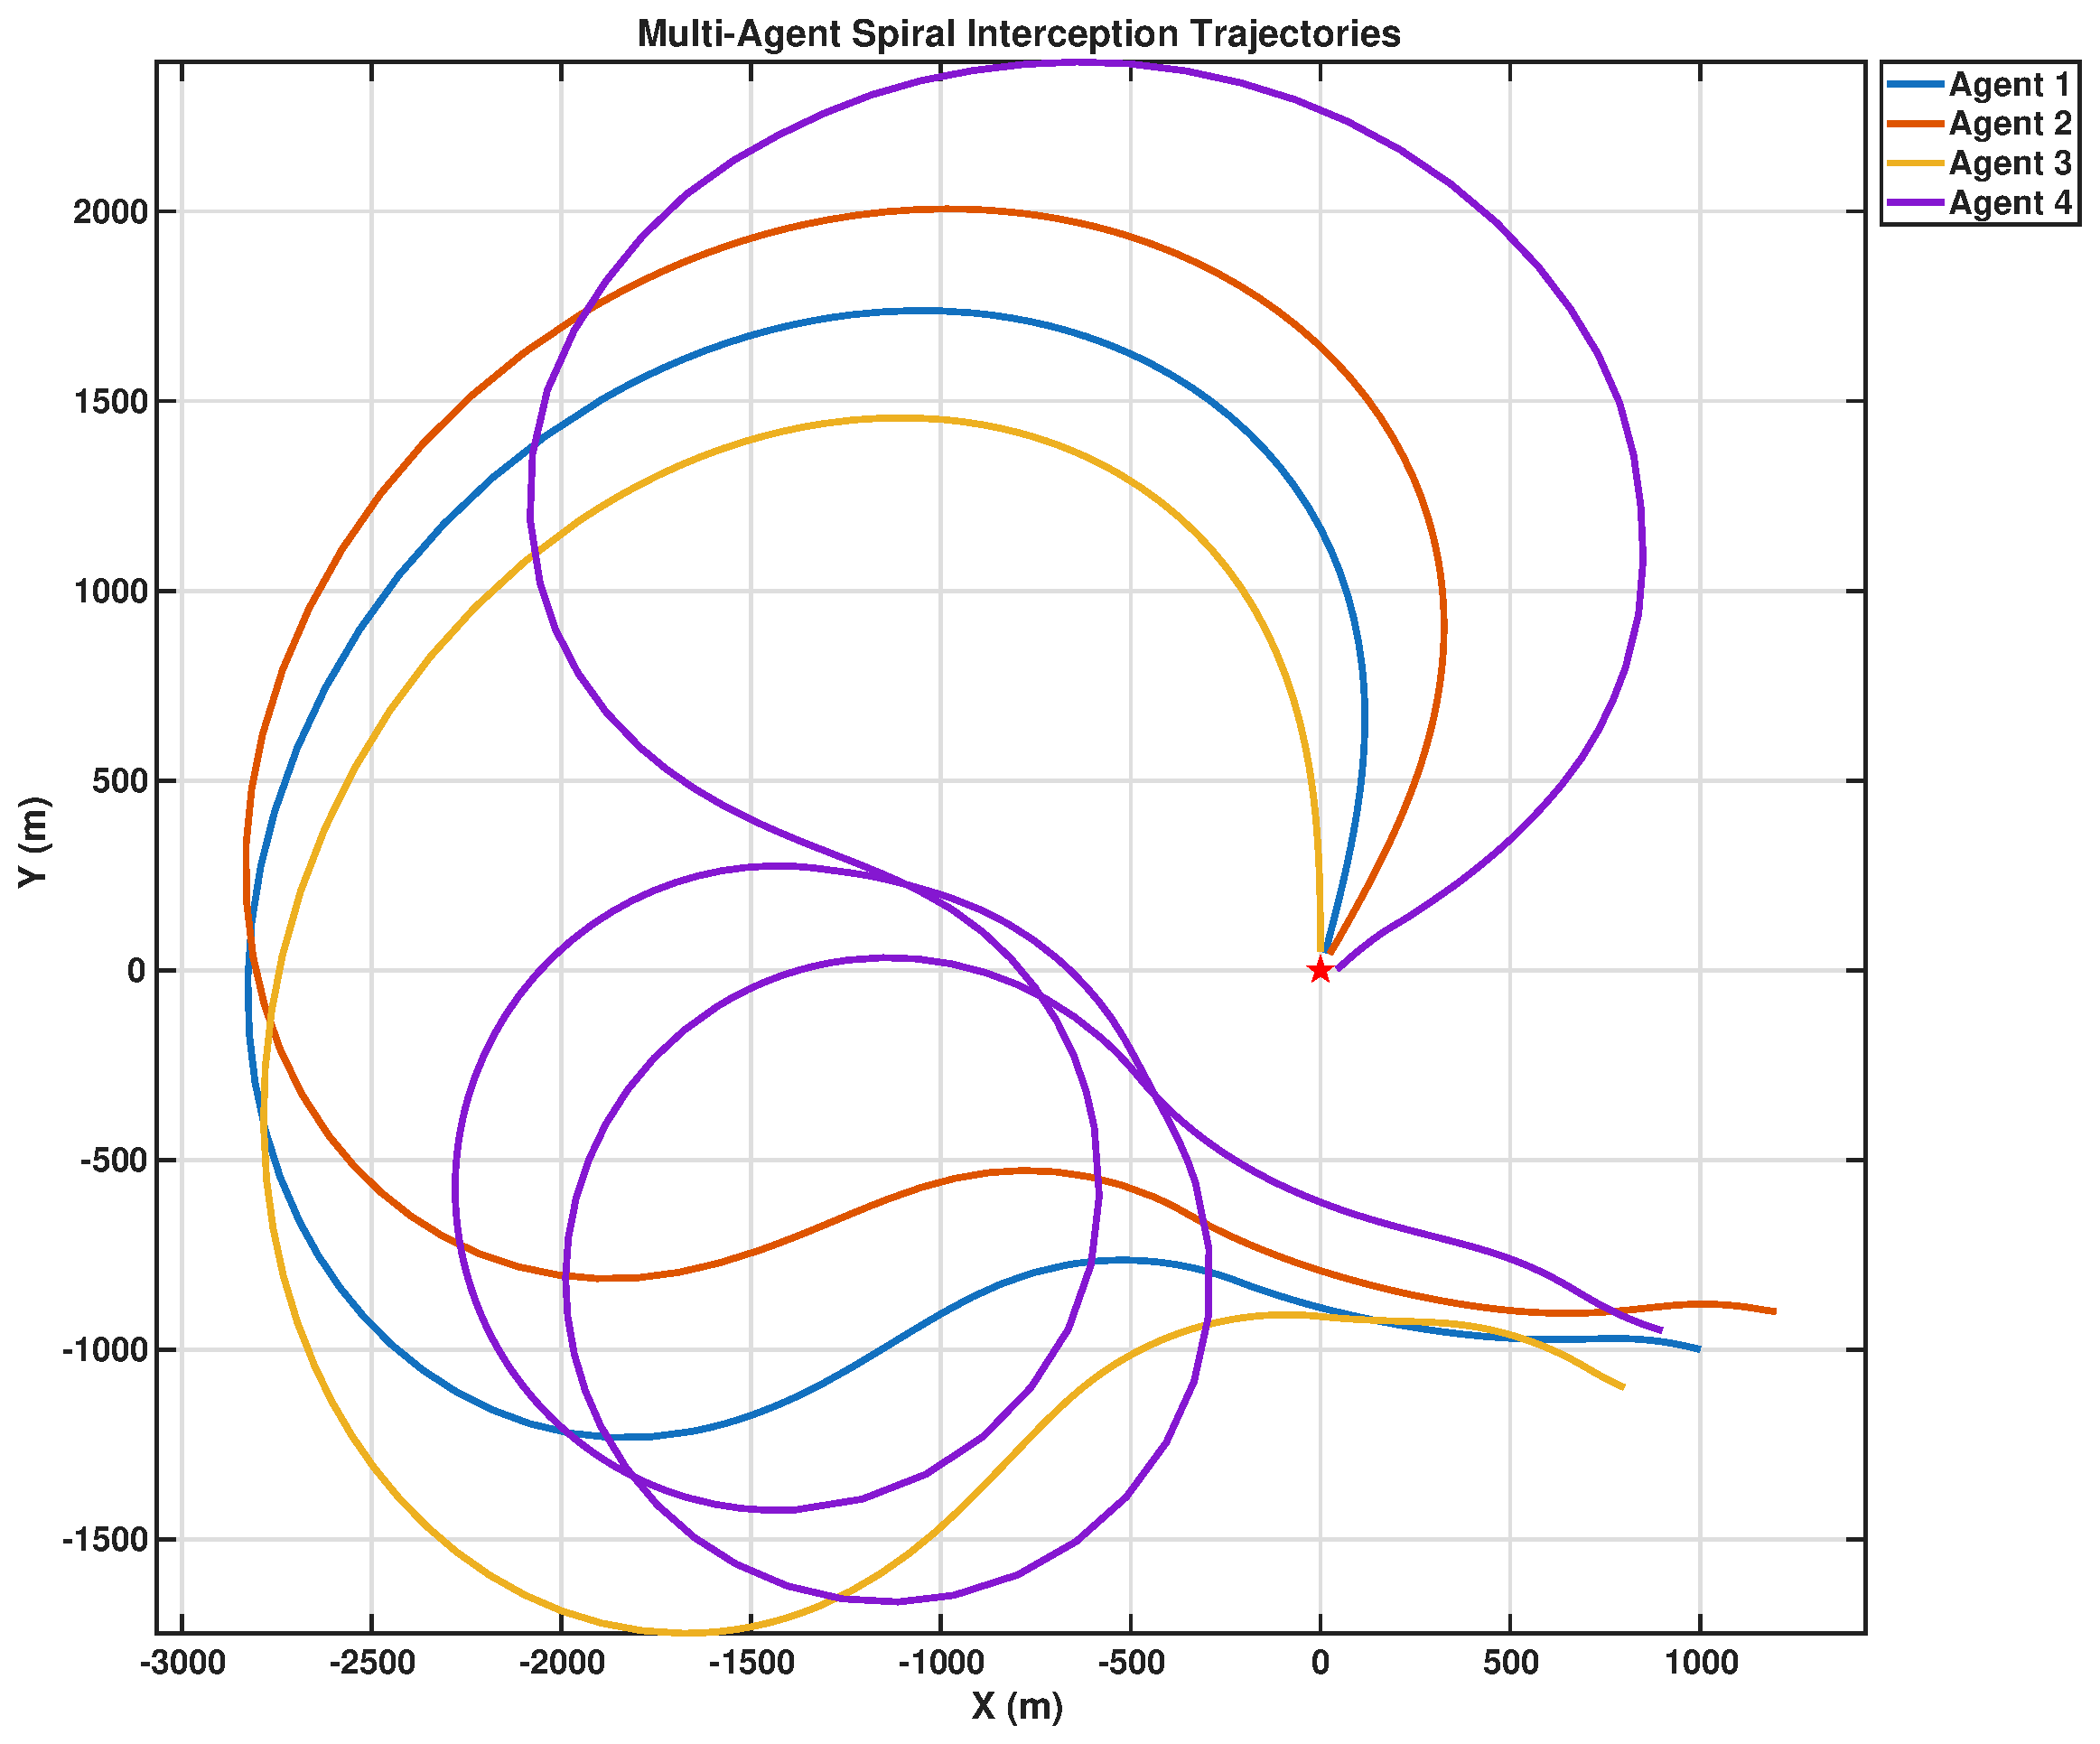
\includegraphics[width=0.75\textwidth]{6_Images/4Agent_Case2_Trajectory.eps}
	\caption{Spatial interception trajectories for $N=4$ pursuers under a shifted impact sector ($\Delta \zeta = \pi/3$).}
	\label{fig:ch_sp_4agent_case2_traj}
\end{figure}

As shown in Figure~\ref{fig:ch_sp_4agent_case2_traj}, despite the severe angular shift requiring extensive initial heading reorientation, the cooperative guidance law automatically re-routes the spatial trajectories. All four pursuers successfully absorb the large initial line-of-sight errors without encountering actuator saturation ($|a_{p,i}(t)| \le 30g$), achieving simultaneous target impact at the shifted approach angles.
\subsubsection{Case 3: Fleet Scalability Evaluation ($N = 5$ Agent)}\label{subsubsec:ch_sp_5agent_case7}
To confirm scalability for larger multi-agent formations, a fleet of $N = 5$ pursuers was evaluated under a dense sector allocation $\zeta_i \in [-80^\circ, 40^\circ]$.

\begin{figure}[!ht]
	\centering
	\begin{subfigure}[b]{\textwidth}
		\centering
		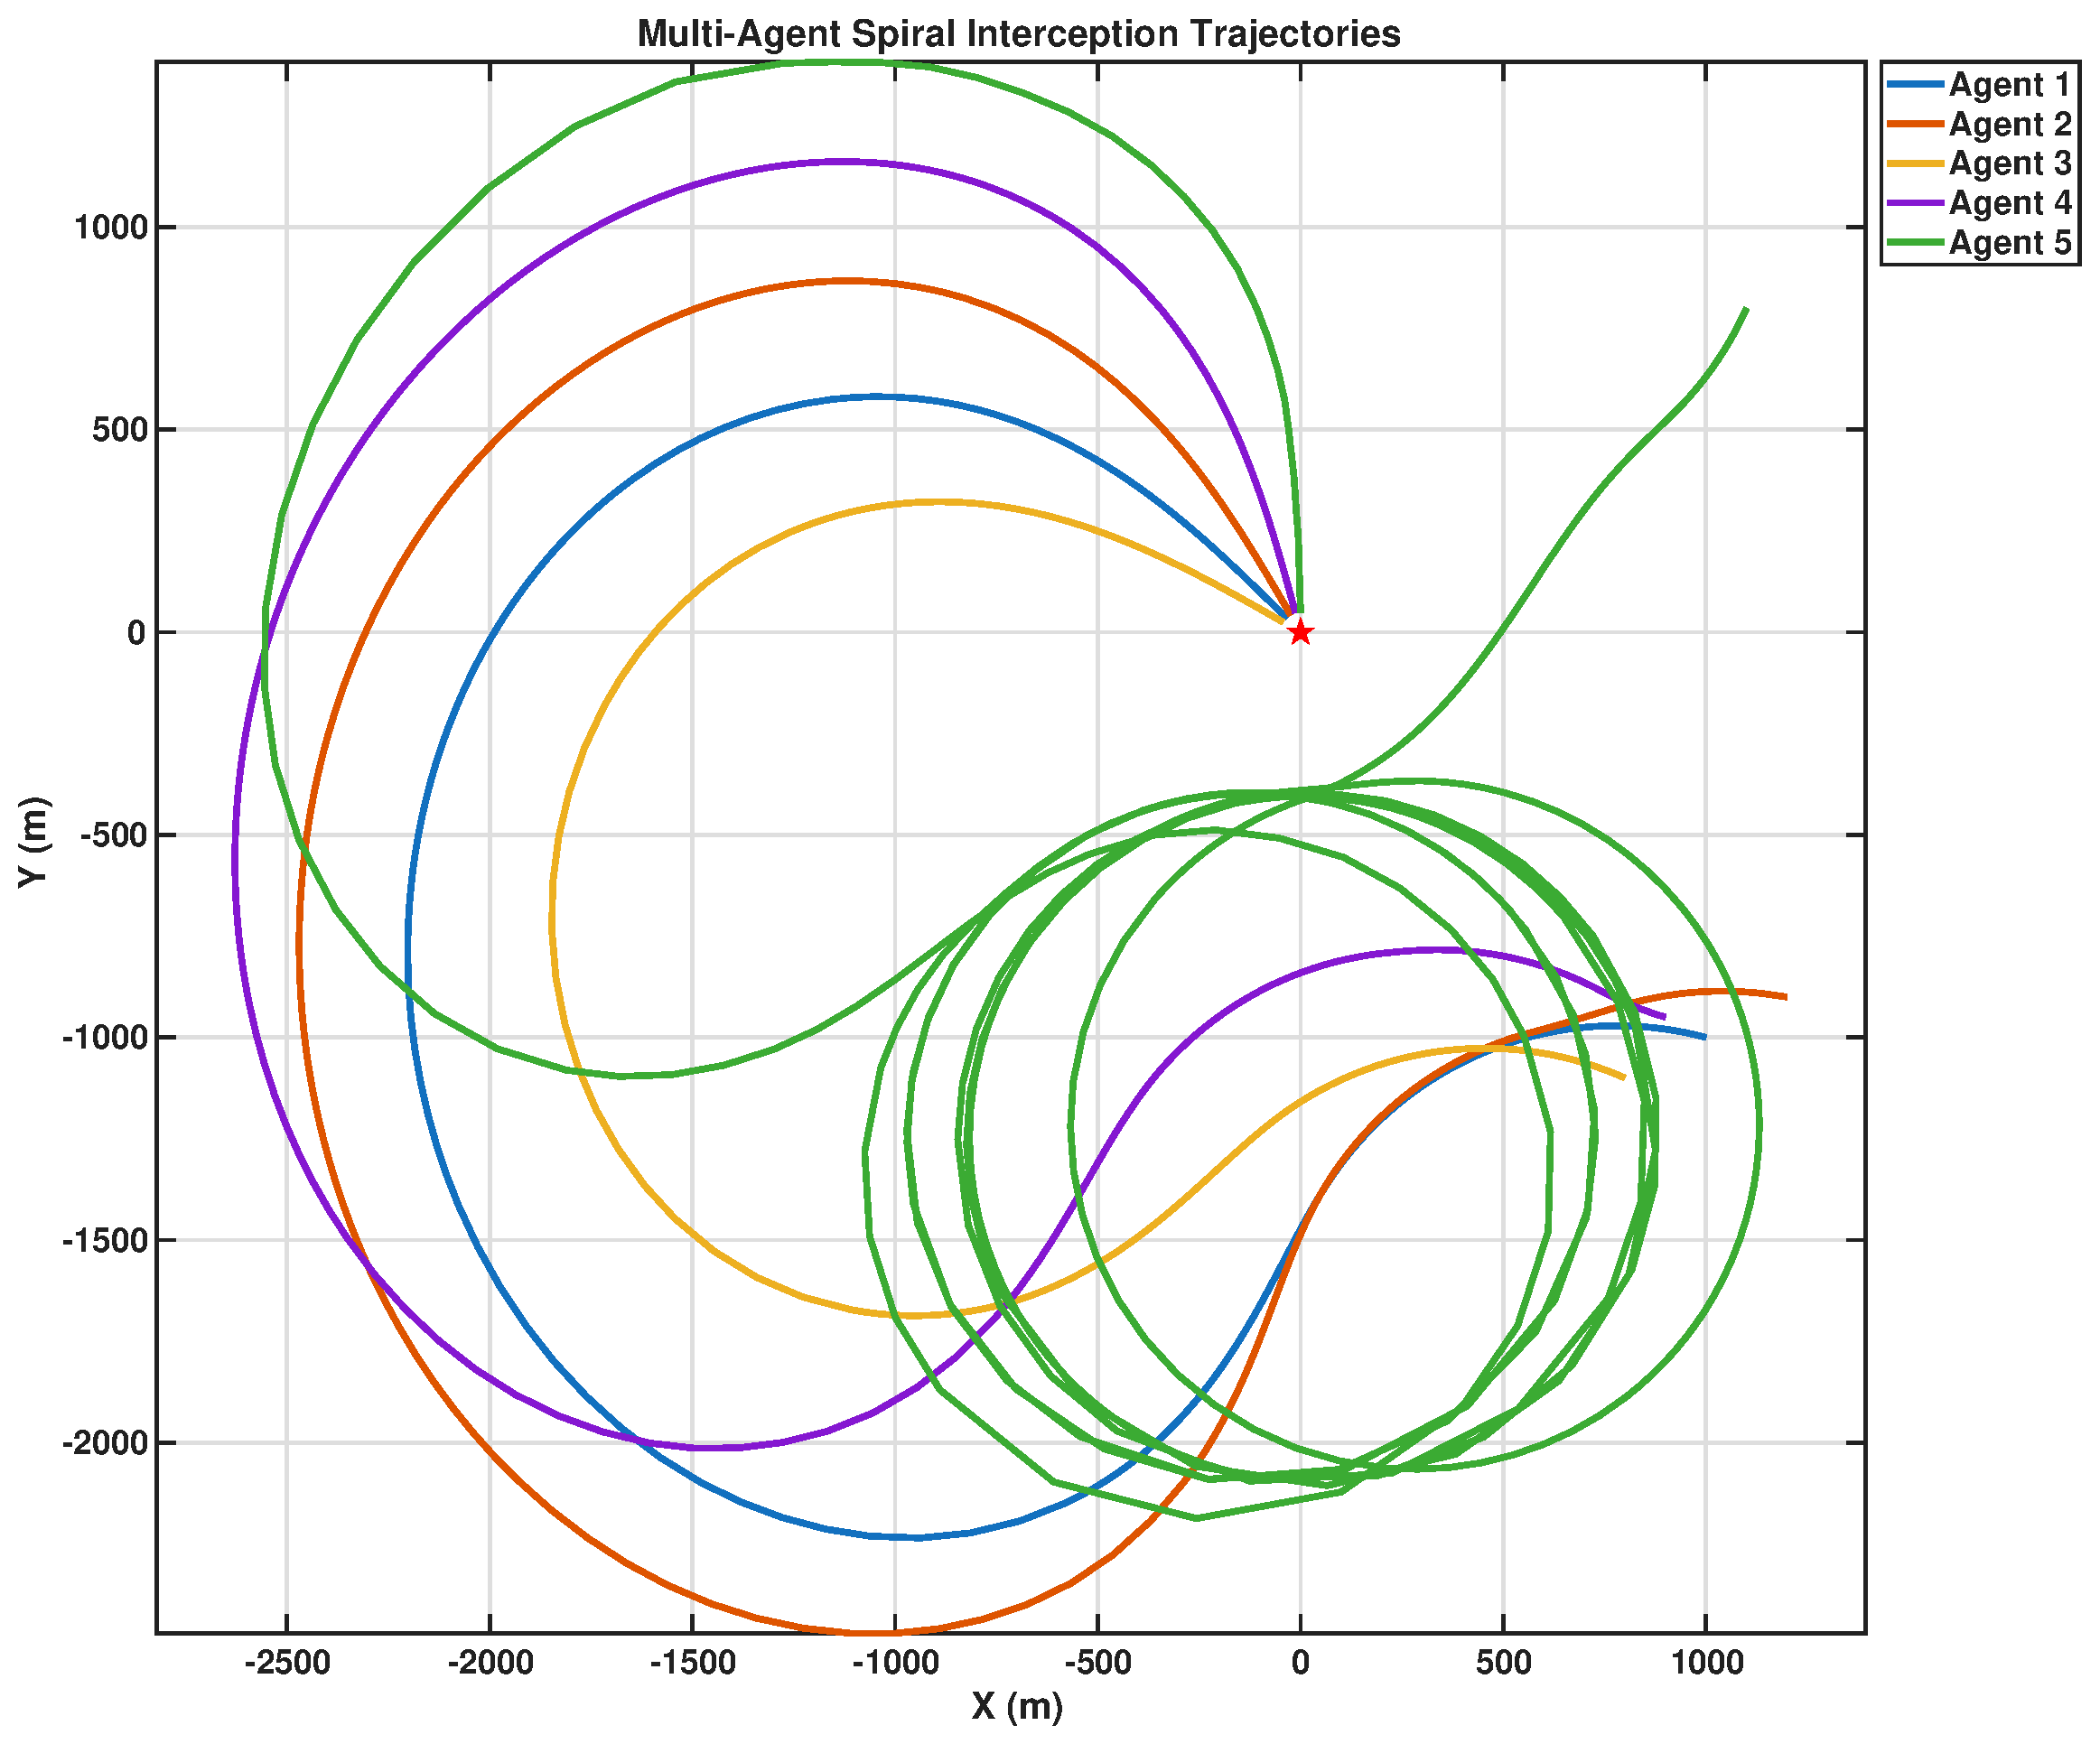
\includegraphics[width=0.8\textwidth]{6_Images/4Agent_Case7_Trajectory.eps}
		\caption{Spatial interception trajectories ($N=5$).}
		\label{fig:ch_sp_5agent_case7_traj}
	\end{subfigure}
	\hfill
	\begin{subfigure}[b]{\textwidth}
		\centering
		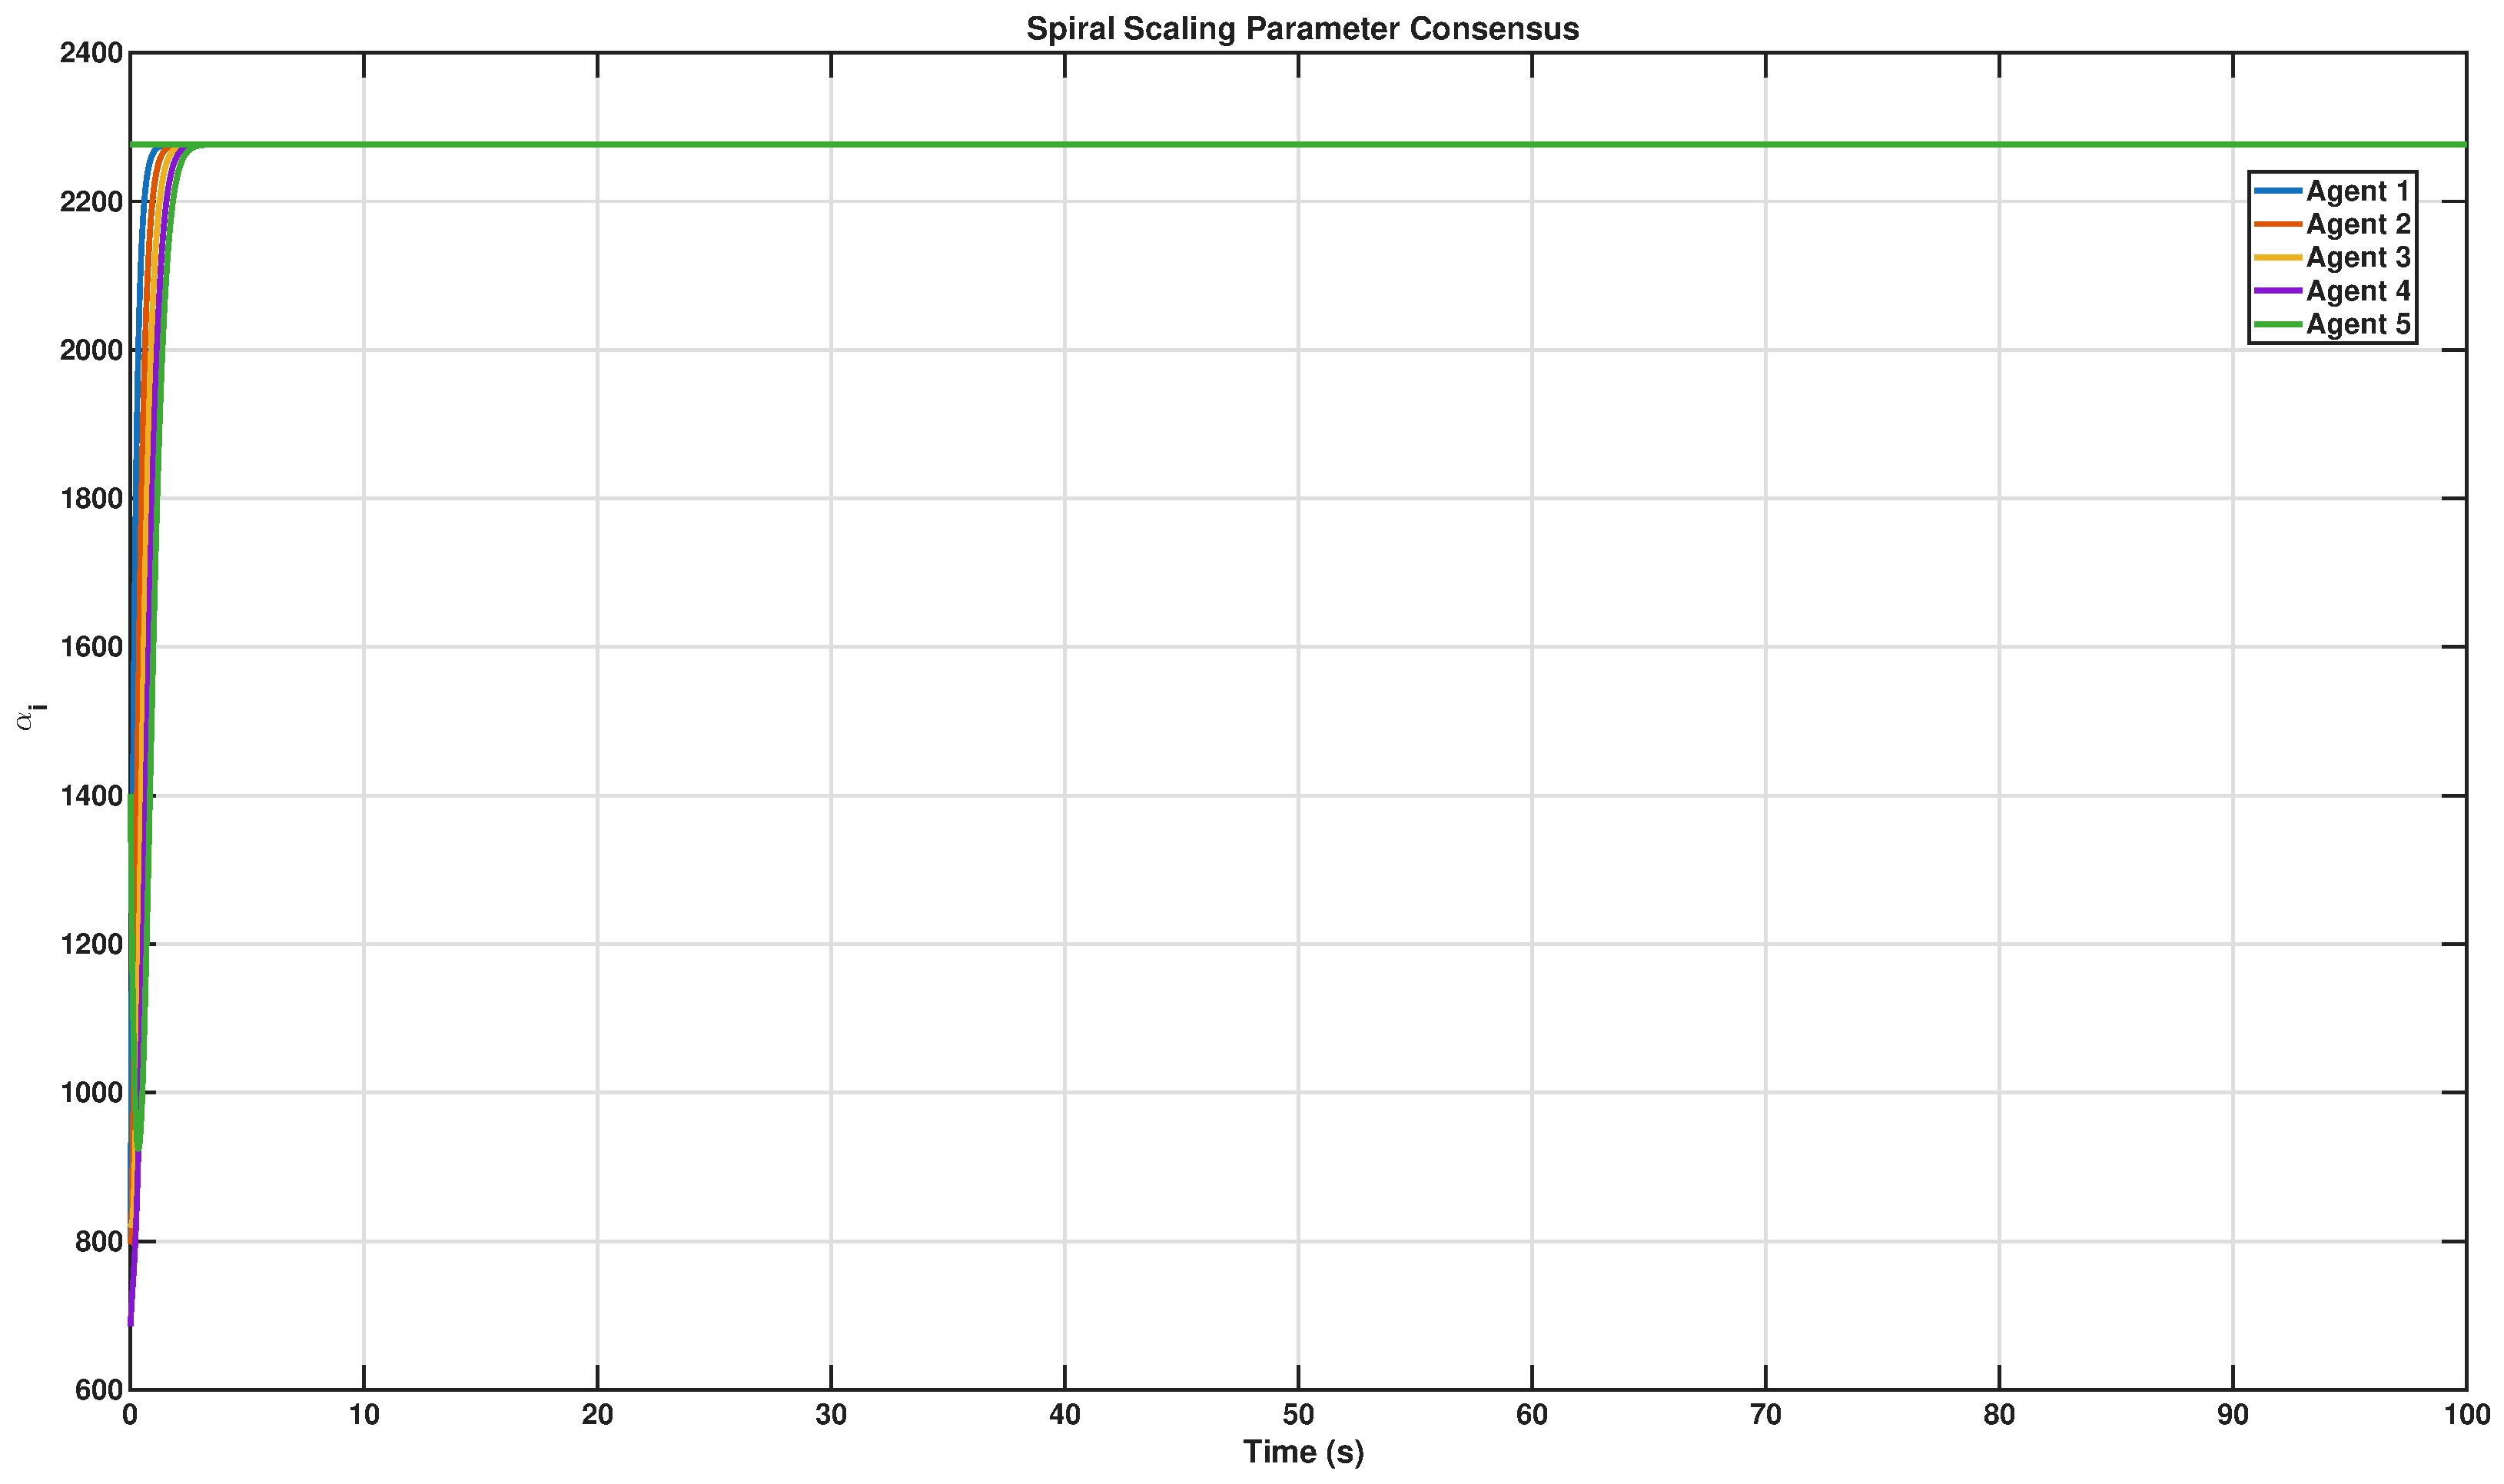
\includegraphics[width=0.8\textwidth]{6_Images/4Agent_Case7_Alpha_Evolution.eps}
		\caption{Consensus evolution of scaling parameters $\alpha_i(t)$.}
		\label{fig:ch_sp_5agent_case7_alpha}
	\end{subfigure}
	\caption{Multi-agent cooperative interception ($N=5$) demonstrating fleet scalability and robust consensus convergence.}
	\label{fig:ch_sp_5agent_sim7}
\end{figure}

Figures~\ref{fig:ch_sp_5agent_case7_traj} and \ref{fig:ch_sp_5agent_case7_alpha} confirm that fleet expansion does not induce control degradation or network instability. The five scaling parameters $\alpha_i(t)$ achieve uniform consensus at $\alpha_{\text{ref}} = 1241.5$ within $1.15\text{ s}$, while the spatial trajectories show uniform angular distribution around the target origin, verifying the algorithm's viability for high-density multi-agent operations.
\section{Summary}\label{sec:ch_sp_summary}

In this chapter, a two-phase adaptive guidance law and multi-agent coordination protocol was developed using generalized Archimedean spirals:
\begin{itemize}
	\item \textbf{Curvature Feasibility Threshold:} We derived exact closed-form expressions for maximum spiral curvature $\kappa_{\max} = f(\beta)/\alpha$, establishing reference threshold $\alpha_{\text{ref}} = v_p^2 f(\beta)/a_{\max}$ to prevent lateral acceleration saturation.
	\item \textbf{Two-Phase Adaptive Control:} Phase 1 adapts $\alpha(t) \to \alpha_{\text{ref}}$ dynamically under prescribed-time error feedback, eliminating control saturation before transitioning to Phase 2 geometric impact angle tracking.
	\item \textbf{Multi-Agent Directed Consensus:} Directed graph consensus over vector $\boldsymbol{\alpha}$ achieves synchronized, sector-allocated coordinated interception across heterogeneous pursuer fleets.
\end{itemize}